%%%%%%%%%%%%%%%%%%%%%%%%%%%%%%%%%%%%%%%%%%%%%%%%%%%%%%%%%%%%%%%%%%%%%%%
%                                                                     %
%    LateX template for UG final report                               %
%    S.S. Oyelere
%    Feb 2025
%    University of Exeter                                             %
%                                                                     %
%%%%%%%%%%%%%%%%%%%%%%%%%%%%%%%%%%%%%%%%%%%%%%%%%%%%%%%%%%%%%%%%%%%%%%%
\documentclass[11pt,a4paper]{article}

\usepackage{amsmath}
\usepackage{amsfonts}
\usepackage{geometry}
\usepackage{graphicx}
\usepackage{url}
\usepackage{fancyhdr}
\usepackage{setspace}
\usepackage{amssymb}
\usepackage{booktabs}
\usepackage{enumitem}
\usepackage{multirow}
\usepackage{titlesec}
\usepackage{placeins}
\usepackage[font=footnotesize]{caption}

% open up the gap before a top-level section, so a new study is visibly
% separated from the end of the previous one. Subsections keep their defaults.
\titlespacing*{\section}{0pt}{7ex plus 1.5ex minus .5ex}{2.3ex plus .2ex}

% set table of content depth
\setcounter{tocdepth}{3}
\usepackage[titles]{tocloft}

% set spacing
\setlength{\cftbeforesecskip}{10pt}

% Page layout settings
\geometry{
    a4paper,
    left=20mm,
    right=20mm,
    top=25mm,
    bottom=25mm
}

%%%%%%%%%%%%%%%%%%%%%%%%%%%%%%%%%%%%%%%%%%%%%%%%%%%%%%%%%%%%%%%%%%%%%%
%%%%%%%%%%%%%%%%%%%%%%%%%%%%%%%%%%%%%%%%%%%%%%%%%%%%%%%%%%%%%%%%%%%%%%
\begin{document}
\singlespacing  % Set the document to single line spacing
\thispagestyle{empty} % remove page number for the cover page

\begin{center}
{\bf \LARGE The Communication Tax: Isolating and Scaling the Coordination Costs of Multi-Agent LLM Coding Systems}\\[0.5cm]
    \textbf{Your Name} \\[0.2cm]
    \textbf{Student ID:} 1234567890 \\[1cm]
    % \textbf{Email:} youremail@exeter.ac.uk \\[1cm]
\end{center}

\section*{Abstract}

\noindent
Multi-agent LLM systems promise the parallelism and division of labour of human teams, but whether coding agents can actually coordinate on shared codebases is largely untested. We first replicate CooperBench's ``curse of coordination'' on our own infrastructure with a stronger, paired design: on 46 matched feature pairs with an identical model (Claude Sonnet 5), a solo agent's pass rate of 44.2\% falls to 12.3\% when two agents must coordinate via free-text messaging (Wilcoxon $p < .001$). Per-feature evaluation localises the gap: paired agents pass their own feature's held-out suite exactly as often as solo agents (21/47 vs 20/47), and every jointly-failed pair that was individually solvable was lost to a textual merge conflict. Normalising for computational effort widens the gap further, from 3.6-fold in pass rate to 6.3-fold in passes per dollar. We then extend the benchmark into a controlled scaling study: a solo-achievable workload of $K$ mutually conflicting features is held fixed while only the team size $N \in \{1, 2, 3, 4\}$ varies, with integration performed by the agents themselves. Adding agents buys no correctness. The strict all-pass rate falls monotonically from 89\% to 69\% --- while cost rises faster than the work is divided, so efficiency collapses as a power law, $\approx 1.28 \cdot N^{-1.61}$, reaching ${\sim}10\%$ of the solo value at four agents. The collapse is universal across all fourteen task pools, including those that integrate perfectly at every $N$. Finally, we test whether hierarchy escapes this tax: replacing the flat peer topology with a supervisor--worker one --- a supervisor that plans the decomposition, allocates features, and performs the team's single integration --- flattens the cost curve rather than removing the tax. Supervised efficiency falls as $0.63 \cdot N^{-0.69}$ against the flat arm's $N^{-1.61}$, so the two curves cross at ${\approx}2.1$ agents; cost rises by a third across two to five agents where flat peers more than triple across two to four, and the strict correctness rate holds between 76\% and 83\% where flat peers fall monotonically from 89\% to 69\%. Coordination overhead in agentic software development is thus super-proportional in team size under the standard peer topology: a composite tax whose message-independent floor --- the redundant context each agent must load --- is paid before any message is sent, with messaging and the rework it triggers adding roughly a third more on top. Hierarchy does not remove the tax, but centralising allocation and integration flattens its growth enough that supervision dominates flat peers from three agents up --- while still never beating one agent working alone.

%
\newpage
\thispagestyle{empty}
\section*{Declaration}
I acknowledge the following uses of GenAI tools in this assessment:


\begin{itemize}[label={\ $\square$\ }, leftmargin=*]

% To tick the boxes, set the label value as follows
% \begin{itemize}[label={\ $\text{\rlap{$\checkmark$}}\square$\ }, leftmargin=*]

  \item I have used GenAI tools to:
  \begin{itemize}[label={\ $\square$\ }, leftmargin=*]
    \item develop ideas.
    \item assist with research or gathering information.
    \item help me understand key theories and concepts.
    \item identify trends and themes as part of my data analysis.
    \item suggest a plan or structure for my assessment.
    \item give me feedback on a draft.
    \item generate images, figures or diagrams.
    \item proofread and correct grammar or spelling errors.
    \item generate citations or references.
    \item Other: [please specify]
    \item[]
  \end{itemize}

  \item I have not used any GenAI tools in preparing this assessment.
\end{itemize}

\bigskip
I declare that I have referenced all use of GenAI outputs within my assessment in line with the University referencing guidelines.

\vspace{1em}
I certify that all material in this dissertation which is not my own has been identified.

\vspace{5em}
{\bf\noindent Signature:} \hrulefill
\newpage


% table of contents
\tableofcontents
\thispagestyle{empty}
\newpage

% reset page number
\clearpage
\pagenumbering{arabic}
%%%%%%%%%%%%%%%%%%%%%%%%%%%%%%%%%%%%%%%%%%%%%%%%%%%%%%%%%%%%%%%%%%%%%%
%
%    Introduction and Related Literature
%
%%%%%%%%%%%%%%%%%%%%%%%%%%%%%%%%%%%%%%%%%%%%%%%%%%%%%%%%%%%%%%%%%%%%%%
\section{Introduction and Related Literature}\label{sec:intro}

Large language models (LLMs), when given a sequence of text, predict the continuation token by token. LLMs retain no memory from one run to the next --- they are stateless. An AI agent is what emerges when an LLM is wrapped in a loop --- given a ``harness''. The agent is provided with access to tools, allowing it to execute against a real environment. The resulting output is fed back into the agent's context, giving it a working memory across steps --- a state. This infrastructure turns a next-token predictor into a system that can pursue multi-step goals such as editing files and reading a codebase~\cite{yang2024sweagent}, surfing the internet~\cite{yao2022webshop} or managing databases~\cite{pourreza2023dinsql}.

The concept of a multi-agent system itself is not novel; discussion of such systems goes as far back as the late 1970s, and can be seen in Hewitt's model of intelligence as a ``society'' of communicating problem-solving experts (Artificial Intelligence, 1977)~\cite{hewitt1977control}. For the sake of simplicity, in this paper, an ``agent'' will always be referring to an LLM-based agent.

After one has realised the benefits of a single agent, the appeal for a team of several is obvious, and multi-agent systems have risen in popularity accordingly. The intuition borrows from human organisations: divide the work, letting multiple workers share the load and collaborate. In theory, several agents should provide the parallelism that a single model instance cannot. Frameworks built on this premise have proliferated, from conversational multi-agent toolkits such as AutoGen~\cite{wu2023autogen} to software company simulations such as MetaGPT~\cite{hong2023metagpt} and ChatDev~\cite{qian2024chatdev}, which spawn teams of agents with focused tasks such as engineers, testers and product managers.

Popular frameworks for orchestrating these agents have risen in popularity alongside them, differing mainly in how coordination is expressed. Google's Agent Development Kit (ADK)~\cite{google2025adk} arranges agents into a hierarchical tree, while LangChain~\cite{chase2022langchain} and its graph-based successor LangGraph~\cite{langchain2024langgraph} provide infrastructure for building complex multi-agent systems with explicit state management and graph-based architectures. CrewAI~\cite{crewai} assigns agents named roles within a ``crew'', closely mirroring the divide-the-work intuition described above. The OpenAI Agents SDK~\cite{openai2025agents} instead coordinates through explicit handoffs, and the Claude Agent SDK~\cite{anthropic2025claudesdk} through delegation to sub-agents. Parallel to these engineering efforts, a new research line has emerged, studying agent collaboration directly, including CAMEL~\cite{li2023camel} on role-playing communication and AgentVerse~\cite{chen2023agentverse} on emergent behaviour in agent groups.

Each of these, however, relies on the same intuition --- dividing work provides additional benefit. In ``CooperBench: Why Coding Agents Cannot be Your Teammates Yet''~\cite{khatua2026cooperbench}, Khatua et al.\ found that solo agents solved coding tasks at substantially higher rates than their multi-agent counterparts. ``The curse of coordination'' (fittingly named by the authors) suggests agents average ${\sim}30\%$ lower success working together than one agent doing both tasks alone. Similarly, Cemri et al.\ (2025)~\cite{cemri2025why} observe that multi-agent system performance gains, across popular benchmarks, remain minimal when compared to single-agent frameworks. The authors analyse over 200 tasks across seven popular multi-agent frameworks and identify fourteen recurring failure modes. The failures demonstrate structural consequences of coordination, suggesting that the overhead introduced by dividing work between agents can actively erode the capability of the underlying model. Comparable findings emerge even in the narrower setting of multi-agent debate, one of the most widely adopted collaboration patterns. Smit et al.\ (2024) benchmark a range of debate protocols against single-model prompting strategies and find that debating systems, in their current form, do not reliably outperform simpler alternatives such as self-consistency, despite incurring considerably greater cost in tokens and latency. Where debate protocols did recover performance, it was only after careful hyperparameter tuning~\cite{smit2024mad}.

So where are they going wrong? To crudely understand the cost of team scaling, one must consider two fundamental properties of communication. Firstly, the re-ingestion of context --- sharing information with another agent means compounding the total system context size. Secondly, and to further compound, messages may be overworded, inconclusive or incorrect --- a greater proportion of messaging increases the chance for misinformation to be spread. Decisions that a solo agent would make alone against a coherent whole are instead made against a fragmented many. Consequently a multi-agent system will often spend more to reach the same outcome. Surely no amount of additional tuning or structural design can recover the coherence a single context provides. In this paper, we refer to the compound communication overhead as the ``Communication Tax''.

Why then would we consider improving a system that is doomed to underperform? Ultimately, efficiency and success rate are not the only measures of value. Multi-agent systems, despite being less effective, may at times be more useful or perhaps necessary. Some tasks pair agents with contrasting abilities~\cite{lowe2017maddpg}, and in other settings, agents may be forced to work together whether or not collaboration is optimal~\cite{stone2010adhoc}. When they do, we want to make sure they do so to their maximum capability while paying as little of the ``communication tax'' as possible.

%%%%%%%%%%%%%%%%%%%%%%%%%%%%%%%%%%%%%%%%%%%%%%%%%%%%%%%%%%%%%%%%%%%%%%
%
%    Our Aims
%
%%%%%%%%%%%%%%%%%%%%%%%%%%%%%%%%%%%%%%%%%%%%%%%%%%%%%%%%%%%%%%%%%%%%%%
\section{Our Aims}\label{sec:aims}

In this paper, we aim to isolate and measure the communication overhead (``Communication Tax'') in multi-agent systems and, through contributions to benchmarking apparatus and additional experiments, quantify how changes in team size and structure affect the tax. We hypothesise that multi-agent systems will typically underperform their solo counterparts in terms of efficiency, primarily due to the growing communication tax as systems scale --- but that focused topology changes could significantly reduce this gap.

%%%%%%%%%%%%%%%%%%%%%%%%%%%%%%%%%%%%%%%%%%%%%%%%%%%%%%%%%%%%%%%%%%%%%%
%
%    Replicating the Curse of Coordination
%
%%%%%%%%%%%%%%%%%%%%%%%%%%%%%%%%%%%%%%%%%%%%%%%%%%%%%%%%%%%%%%%%%%%%%%
\section{Replicating the Curse of Coordination}\label{sec:replication}

\subsection{Terminology}\label{sec:terminology}

\textbf{In this paper we will refer to a ``task'' --- a set of features from one real repository; a ``feature'' --- one unit of that repository's functions, given to an agent as a natural-language spec; a ``pair of features'' --- any two features from the same task; a ``pool'' --- a collection of features.}

\subsection{CooperBench}\label{sec:cooperbench}

In ``CooperBench: Why Coding Agents Cannot be Your Teammates Yet'', Khatua et al.\ --- alongside their headline finding of ``The Curse of Coordination''~\cite{khatua2026cooperbench} --- introduce a comprehensive benchmarking suite that isolates communication failures in multi-agent systems, testing whether multiple LLM coding agents can work in parallel on the same codebase. CooperBench works by sequentially running multiple containerised environments within which agents can work in isolation. Each agent is given a spec, access to its own copy of the codebase, and a tool for messaging other agents (from one up to a whole team). The agents can also read files and edit code. They are then tasked with individually implementing their own features.

After the agents have finished working on their features, or the step or time cap has been reached, the features are naively merged. A naive merge is a textual merge: it combines changes based on the lines of code each agent modified, without understanding any of the code's structure or logic. Overlapping edits are flagged as conflicts, while non-overlapping edits are merged automatically (even if they break each other semantically). The merge is performed by CooperBench automatically, in a fresh container isolated from the agents.

An evaluation is then performed --- a clean merge is run against both features' test suites, resulting in a \texttt{both\_passed} \textbf{success} only if both suites pass. If either suite fails we record a \textbf{failure}.

\subsection{Extending the Evaluation}\label{sec:extendedeval}

Our first contribution to the benchmark --- an extended evaluation suite. Testing only after a clean merge fails to separate instances where an agent never solved its feature from one whose work didn't successfully merge. In such cases the original evaluation pipeline does not discriminate between an agent's ability to code and an agent's ability to write code that integrates. We fix this with the addition of pre-merge function testing. Each agent's individual feature is tested against its own test suite in isolation prior to merging with the other agents. Capability and integration are therefore reported separately, giving us finer granularity.

Secondly we introduce improved cost metrics. Cost is taken directly from the \texttt{total\_cost\_usd} field of the Claude Code CLI's terminating result event --- a single figure the CLI computes from the run's input, output, and cache read/write tokens at Anthropic's published list prices. A run's cost is the sum across its participating agents, which we use as a proxy for computational effort. This gives the first of two cost metrics we add to CooperBench's evaluation --- scoring every condition in passes per dollar alongside pass rate. The second metric: each run's total is decomposed into four additive dollar accounts --- context (loading the shared repository and specification), task (implementing), communication (messages sent, received, and re-ingested), and rework (revisions messages provoke) --- so that the coordination overhead can be located. We do so by reconstructing each agent's per-turn history from the harness's execution stream and weighting each account by its token-type list price, so the four figures sum exactly to the run's cost.

% TODO: figure --- diagram of the extended evaluation pipeline (pre-merge suite,
% naive merge, post-merge suite). No image asset is committed for this yet.

\subsection{Methodology}\label{sec:replmethod}

To establish that the coordination gap reported in ``CooperBench: Why Coding Agents Cannot be Your Teammates Yet'' reproduces, we opted to use the 50-pair flash subset of tasks. This subset accounts for 50 of the ``full'' CooperBench dataset's 652 feature pairs, spanning 20 of its 30 tasks and 11 of its 12 repositories. A smaller dataset is selected over a larger one, allowing us to perform multiple passes over the same $N$, feature-pair pairs and thus reducing the effect of LLM stochasticity. Preliminary pilot tests were run to determine a suitable model. Factors to consider were cost, individual model capability, and token throughput --- Claude Sonnet 5 was ultimately selected. The model is accessed through the Claude Code CLI, which CooperBench launches headless inside each agent's container. The experiment was run under two conditions: a Solo condition, in which a single agent implements both features of a pair, and a Co-op condition, in which two isolated agents implement one feature each. The agents may optionally exchange messages via a Redis-backed communication channel. Both conditions are run on the identical set of feature pairs --- every feature pair has one Solo result and one Co-op result. This yields a matched design in which the two settings are compared within each feature pair rather than across aggregate scores, removing variance in task difficulty as a confound.

For our replication of the original study, we opted to use the same ``free-msg'' protocol --- the same default protocol that is both shipped with CooperBench and used in the original ``Curse of Coordination'' study. Each agent's instruction is a single prompt composed of three parts: (1) the feature specification; (2) the submission protocol; (3) the cooperation protocol. In ``free-msg'' the agent is informed of its partner, warned of overlapping features and taught messaging commands. These commands allow the agents to message using shell commands through the Redis-backed communication channel.

\begin{quote}
\footnotesize
\begin{verbatim}
## free-msg

You are **agent1**, working alongside: **agent2**.
Each agent has been assigned a separate feature from the same codebase;
your features may overlap (touch the same files), so coordinate to avoid
clobbering each other's changes.

Available shell commands for cross-agent messaging (Redis-backed inbox,
one inbox per agent):

    coop-send <recipient> "message text here"   # send to a specific peer
    coop-broadcast "message text here"          # send to every other peer
    coop-recv                                   # drain your inbox (prints JSON list)
    coop-peek                                   # number of unread messages
    coop-agents                                 # list every agent id

Recommended workflow:

1. At the start, `coop-broadcast` a short summary of your feature and
   which files you intend to touch.
2. Periodically `coop-recv` to read what your peers have sent -- at
   minimum after major edits and before submitting.
3. If two agents need to modify the same file, coordinate explicitly
   (split the file, agree on one owner, or merge changes).
4. Keep messages short and focused: file names, function names, and
   one-sentence intents are usually enough.

Messages are not magic -- your peers only know what you tell them.
\end{verbatim}
\end{quote}

\subsection{The Findings}\label{sec:replfindings}

Consistent with the reported ``Curse of coordination'', we observe a substantial drop in task success from the solo agent to its two-agent counterpart. Across 46 matched feature pairs (4 runs removed --- intermittent evaluation-container failures left too few scored runs for a reliable estimate) the average pass rate fell from 44.2\% under the Solo condition to 12.3\% under the Co-op condition --- a reduction of 31.9\%. This finding replicates those of the original study, in which Co-op performance is substantially lower than Solo performance. Recall ``agents average ${\sim}30\%$ lower success working together than one agent doing both tasks alone''~\cite{khatua2026cooperbench}.

In the Co-op condition, both agents' independent work passed their own test suites in 62 of 138 runs (44.9\%) --- statistically indistinguishable from the 61 of 138 runs (44.2\%) passed by the Solo condition. Splitting the work across agents therefore causes no measurable loss of individual capability in the replication. The gap instead arises at patch integration. The agents consistently write working code but cannot place their edits so that contributions cleanly merge with other agents' work. Of the 62 runs where both agents' individual test suites passed, only 17 survived integration, with 45 of the 45 losses due to textual merge conflict.

\subsection{Accounting for Cost}\label{sec:replcost}

CooperBench~\cite{khatua2026cooperbench}, as well as our replication, demonstrates a clear coordination gap in pairs of agents. Earlier we hypothesised that solo agents would be not only more successful but more efficient. We therefore normalise the replication's results by the cost using the new evaluation metric.

Across the same 46 matched feature pairs, the Solo condition achieves 0.675 passes per dollar spent, compared to 0.107 passes per dollar under the Co-op condition --- a 6.3-fold gap, versus the 3.6-fold gap observed in raw pass rate alone. A paired Wilcoxon signed-rank test on per-pair cost efficiency confirms this difference is statistically significant ($W = 2.0$, $p < .001$). This widening indicates that the coordination penalty is not limited to lower success rates: Co-op teams are also less cost-efficient per successful outcome, compounding the disadvantage relative to Solo.

% TODO: figure --- the replication's endpoints (solo vs co-op pass rate and
% passes per dollar). No image asset is committed for this yet.

%%%%%%%%%%%%%%%%%%%%%%%%%%%%%%%%%%%%%%%%%%%%%%%%%%%%%%%%%%%%%%%%%%%%%%
%
%    Scaling The Team
%
%%%%%%%%%%%%%%%%%%%%%%%%%%%%%%%%%%%%%%%%%%%%%%%%%%%%%%%%%%%%%%%%%%%%%%
\FloatBarrier
\section{Scaling The Team}\label{sec:growth}

\subsection{Too Many Cooks}\label{sec:toomanycooks}

In ``Do more agents help? Controlled and protocol-aligned evaluation of LLM agent workflows''~\cite{fu2026agents}, Fu et al.\ find that most multi-agent workflows fail to reliably outperform a matched single-agent baseline once evaluation infrastructure is controlled. They attribute the overall performance to task-protocol fit rather than the number of agents. Their comparison, however, never directly varies agent count independently of communication protocol, prompt, and topology. Similarly, as shown in CooperBench (Khatua et al., 2026)~\cite{khatua2026cooperbench}, coordination performance degrades sharply as the number of cooperating agents increases. In a controlled experiment scaling from 2 to 4 concurrently cooperating agents on 46 tasks drawn from 3 task sets, success rates declined monotonically: from 68.6\% with 2 agents, to 46.5\% with 3 agents, to 30.0\% with 4 agents. This trend reinforces the ``curse of coordination'' observed in the two-agent setting, suggesting that adding more agents to a shared workspace compounds rather than alleviates coordination difficulty.

Again however, their experiment fails to isolate the effect --- agent count is set to the number of features assigned, so a three- or four-agent run carries three or four features. The decline observed therefore confounds coordination overhead with a workload that has grown.

We therefore built PoolBench --- an extension to CooperBench. In PoolBench, the workload is arranged into ``Pools'' comprised of a $K$-feature clique. Each individual pool may be solved by any number of agents $N \in \{1, 2, 3, 4, \ldots, K\}$, allowing us to fix the workload and vary only $N$. All $N$ agents work against one git remote seeded at the feature pool's base commit. Each agent implements its own features, fetches and merges its peers' branches, resolves any conflicts, and rebuilds the patch. Integration is therefore part of the agents' coordination work. The evaluator scores the single integrated tree against each feature's test suite.

\subsection{Methodology}\label{sec:scalingdesign}

\begin{figure}[!ht]
	\centering
	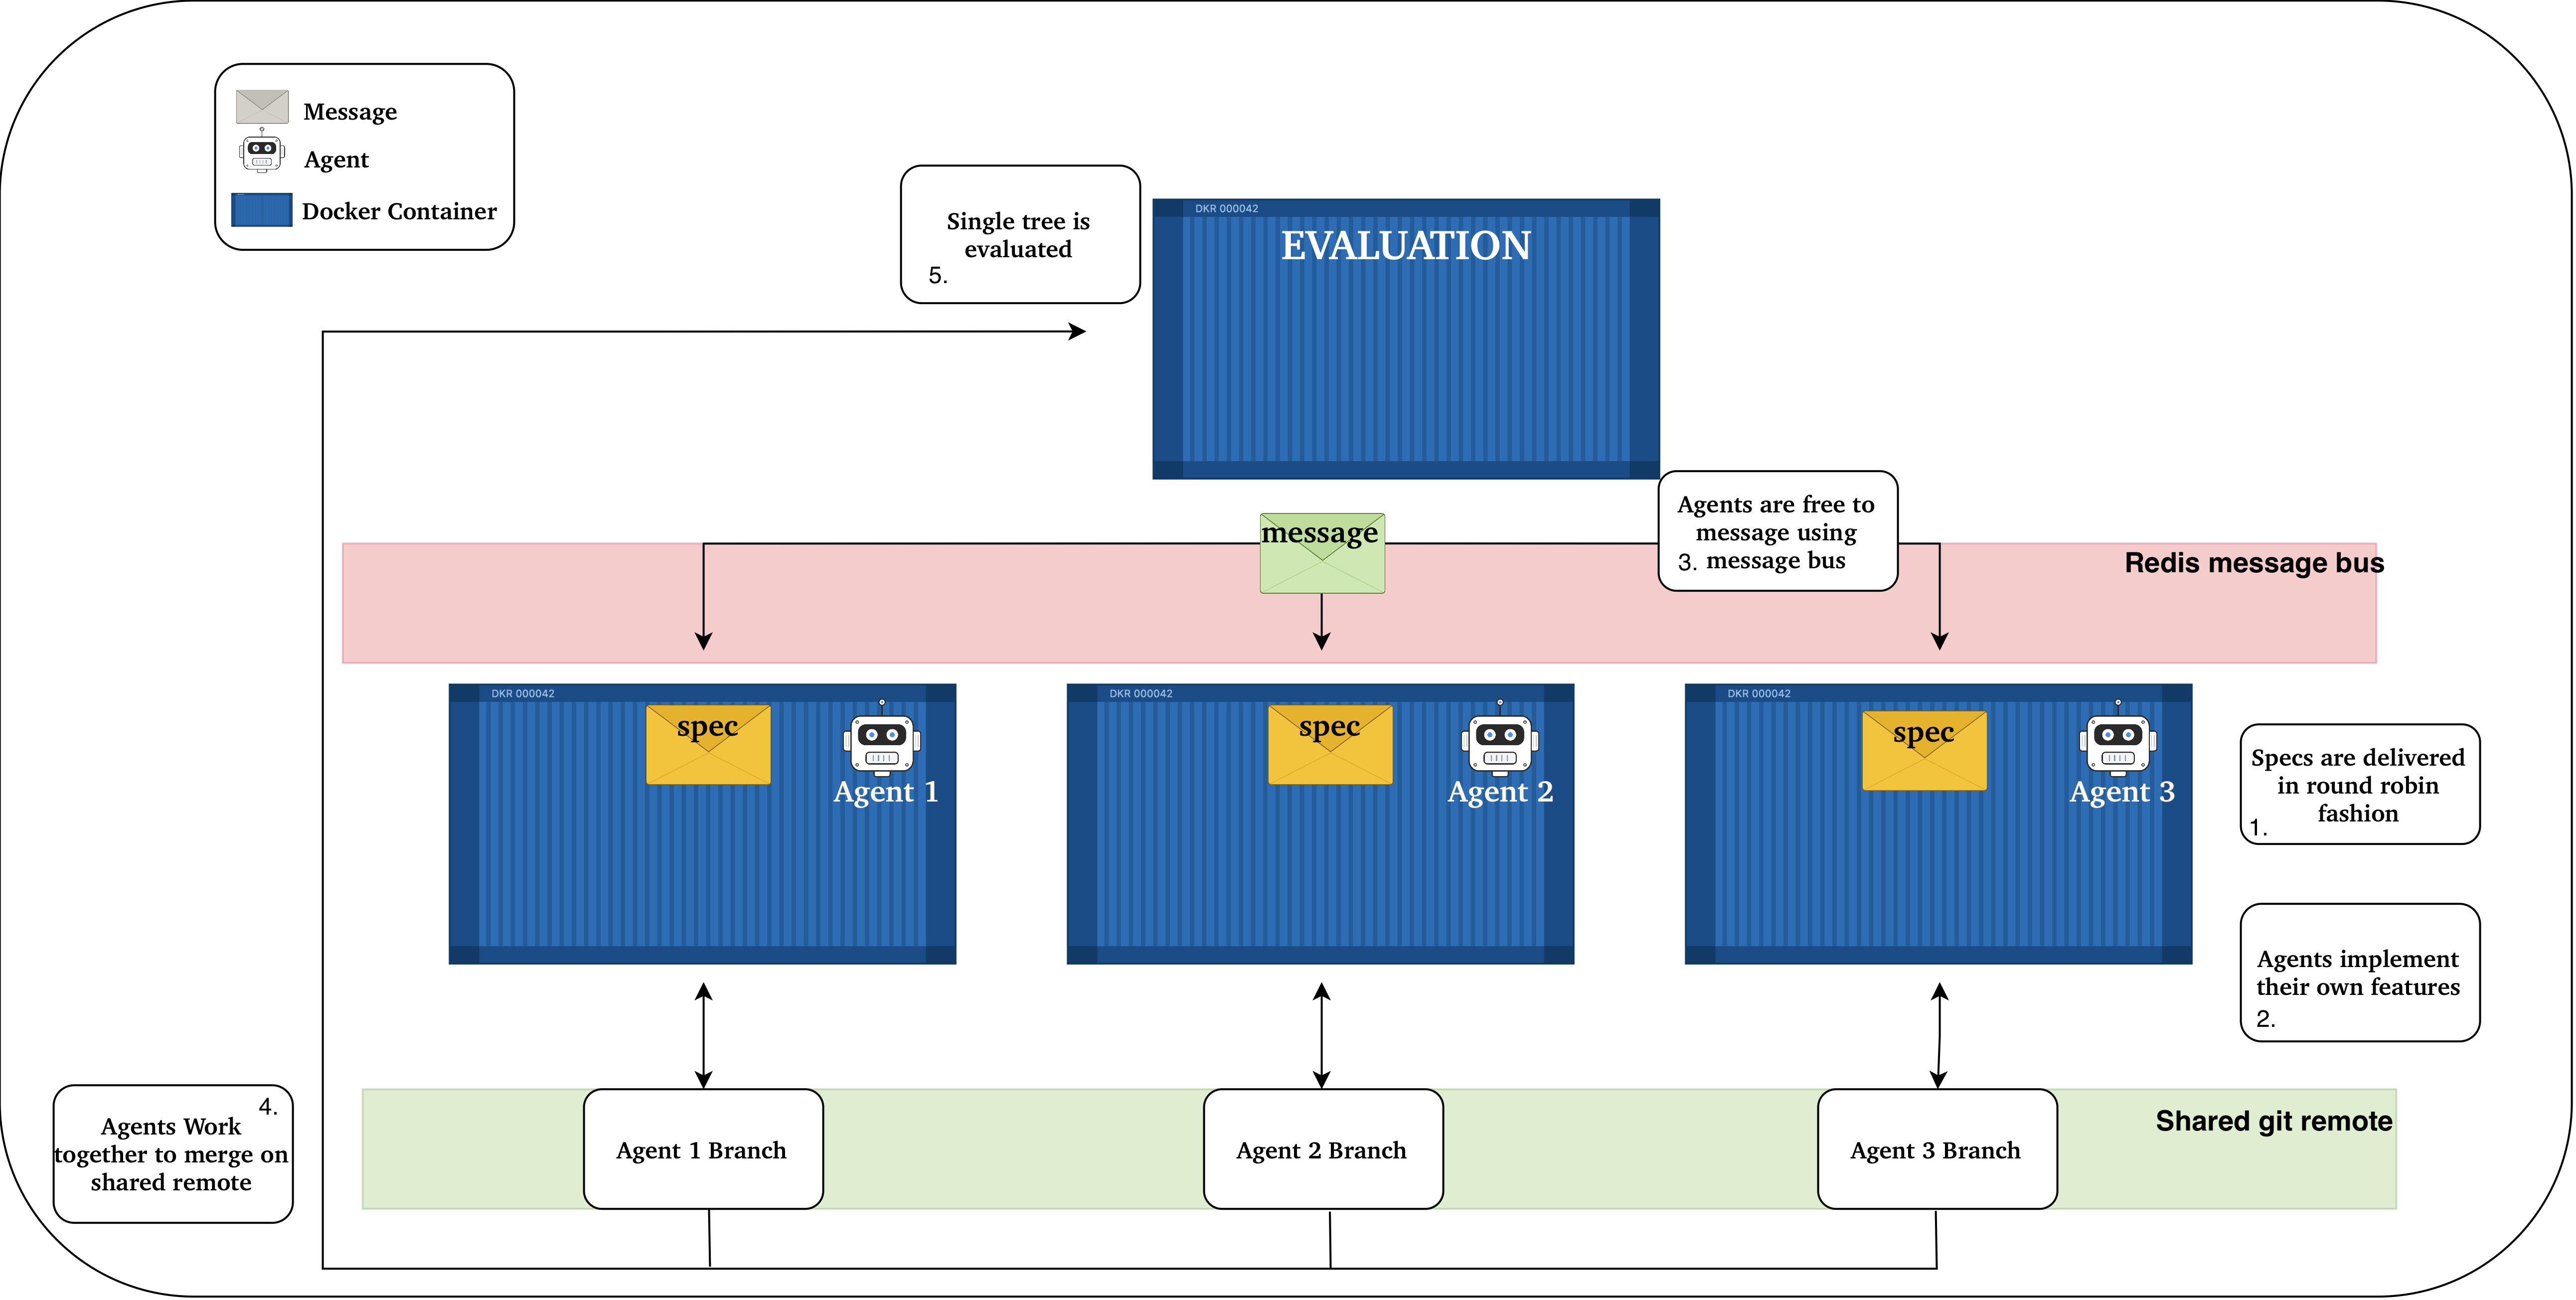
\includegraphics[width=\linewidth]{fig4_flatpeers_architecture.png}
	\caption{\textbf{The flat-peers topology.} (1)~The $K$ specifications are dealt to the agents round-robin; (2)~each implements only its own features; (3)~any agent may message any other over the shared bus; (4)~every agent merges its peers on the shared remote, so integration happens $N$ times; (5)~the resulting tree is scored against all $K$ suites.
    }\label{fig:flatarch}
\vspace{1.2\baselineskip}
\end{figure}

The agents are arranged in a flat-peers topology --- there is no hierarchy between agents (Figure~\ref{fig:flatarch}). The independent variable is $N$ (the number of agents in the team); the constant is the $K$-feature pool. The pool of features is split across the agents using a round-robin distribution as default. Every pool is solo-screened (every pool must be solvable by the solo agent) so that performance losses at higher $N$ can be attributed to coordination cost rather than raw pool difficulty. Primarily we measure a graded score: the fraction of $K$ feature test suites that pass on the integrated tree, allowing us to credit partially correct teams (3/4 features $= 0.75$). The final dataset consists of 14 pools across 6 repositories and 148 total runs using Claude Sonnet 5 (${\sim}\$410$ API-equivalent cost).

\subsection{Results: Efficiency Collapses}\label{sec:poolresults}

\begin{table}[h!]
\centering
\vspace{0.9\baselineskip}
	\caption{Efficiency by agent count $N$, averaged over all pools.\label{tab:efficiency}}
   \renewcommand{\arraystretch}{1.1}
   \setlength{\tabcolsep}{6pt}
\begin{tabular}{ccccc}
 \toprule
 $N$ & Graded score & Cost / run & Solved per \$ & vs.\ solo \\
 \midrule
 1 & 0.96 & \$0.78 & 1.24 & 100\% \\
 2 & 0.91 & \$2.10 & 0.43 & 35\% \\
 3 & 0.89 & \$3.82 & 0.23 & 19\% \\
 4 & 0.92 & \$7.21 & 0.13 & 10\% \\
 \bottomrule
\end{tabular}
\vspace{0.9\baselineskip}
\end{table}

As the number of agents grows, the work solved per dollar collapses, falling as a power law in agent count. Efficiency $= 1.28 \cdot N^{-1.61}$, reaching ${\sim}10\%$ of the solo value at four agents (Figure~\ref{fig:efficiency}). The relationship is universal: fitting each pool separately, all fourteen collapse as power laws with exponents between 1.1 and 2.3. The exponent exceeding 1 across all pools is the substantive point: if dividing the work simply gave each agent a fixed share at a fixed per-agent cost, efficiency would fall as $1/N$, so $b = 1$ is the reference at which coordination itself costs nothing extra. The pooled fit sits well above that reference at $b = 1.61$, and so does every individual pool --- the shallowest of the fourteen still reaches $1.1$ --- so each added agent is super-proportionally wasteful. The coordination tax grows faster than the team grows. This is true even for pools where the correctness never degrades: \texttt{pallets\_jinja/1621} integrates perfectly at every $N$, yet the efficiency falls $1.07 \rightarrow 0.15$, a $7\times$ loss.

\begin{figure}[!htb]
	\centering
	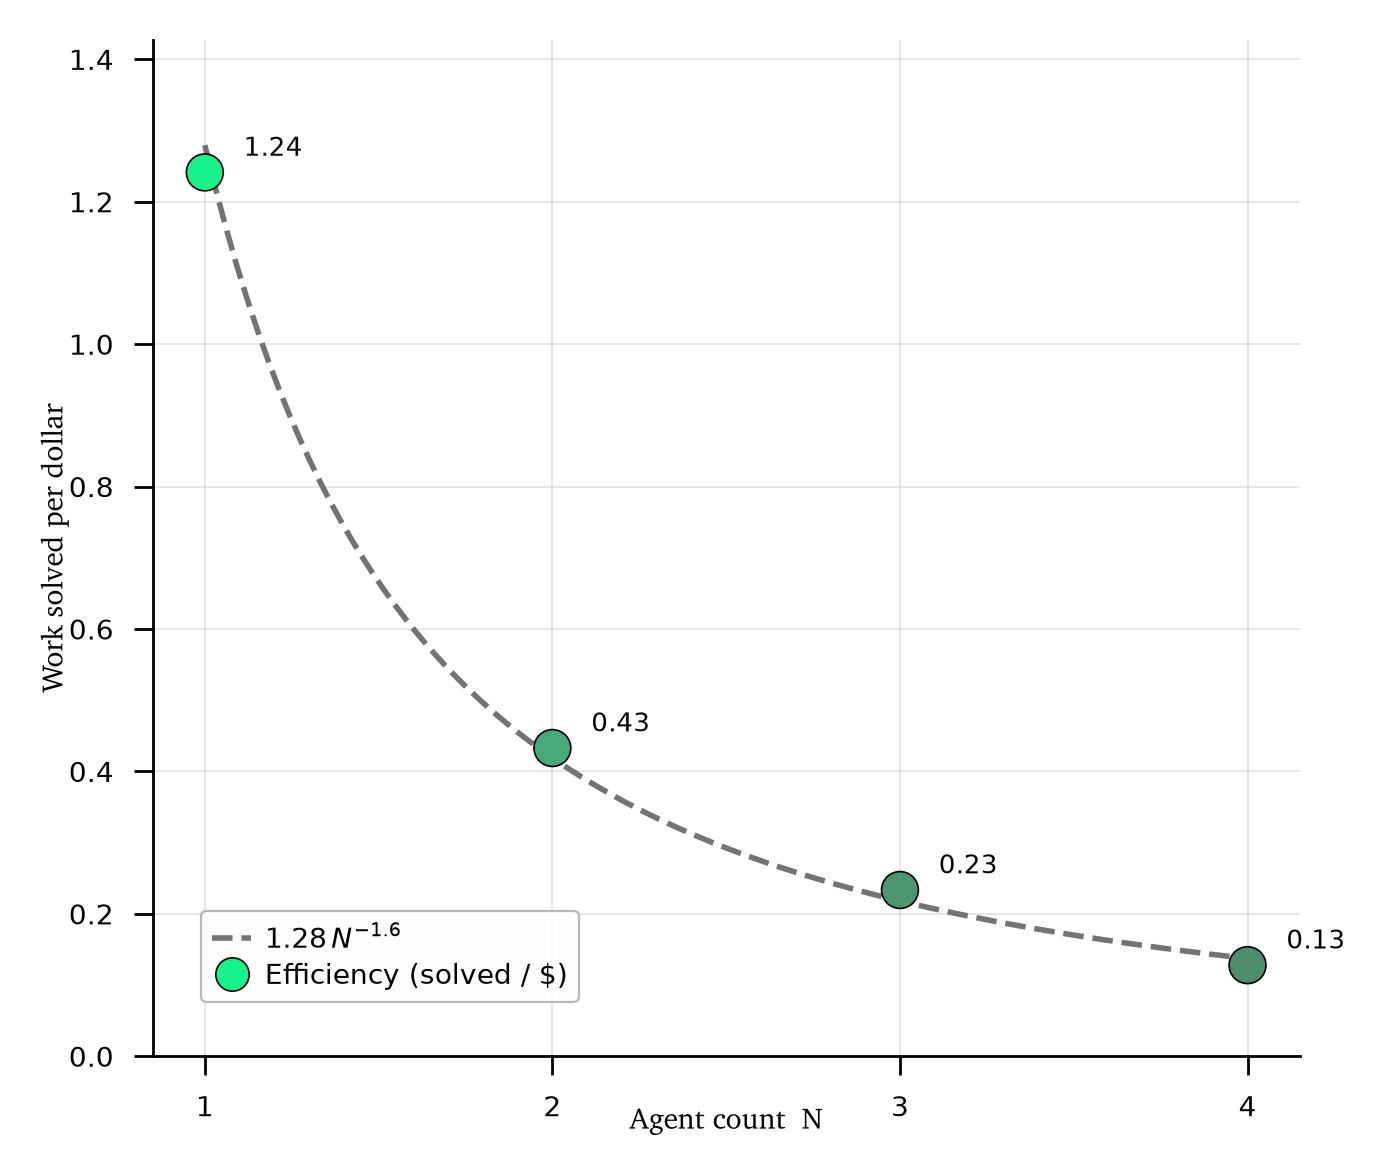
\includegraphics[width=0.6469\linewidth]{fig2c_efficiency.png}
	\caption{\textbf{Efficiency collapses as a power law.} Work solved per dollar falls 1.24 $\rightarrow$ 0.13 across one to four agents, tracking the fitted $1.28 \cdot N^{-1.6}$ (dashed).
    }\label{fig:efficiency}
\end{figure}

\FloatBarrier
\subsection{Results: Correctness Falls More Gradually}\label{sec:scalingcorrect}

Correctness falls more gradually and less universally. The graded score, averaged over all fourteen pools, declines from 0.96 to 0.91 to 0.89 as agent count increases from one to three. Similarly, the strict all-pass rate (the probability the team ships a fully correct integration) falls monotonically from 89\% to 82\% to 77\% to 69\% across one to four agents (Figure~\ref{fig:correctness}). The degradation is concentrated in the hardest repository, \texttt{dspy}: all four of its cliques degrade (e.g.\ $0.75 \rightarrow 0.42$ and $0.92 \rightarrow 0.75$), while eight of the fourteen pools integrate cleanly and remain near 1.0.

\begin{figure}[!htb]
	\centering
	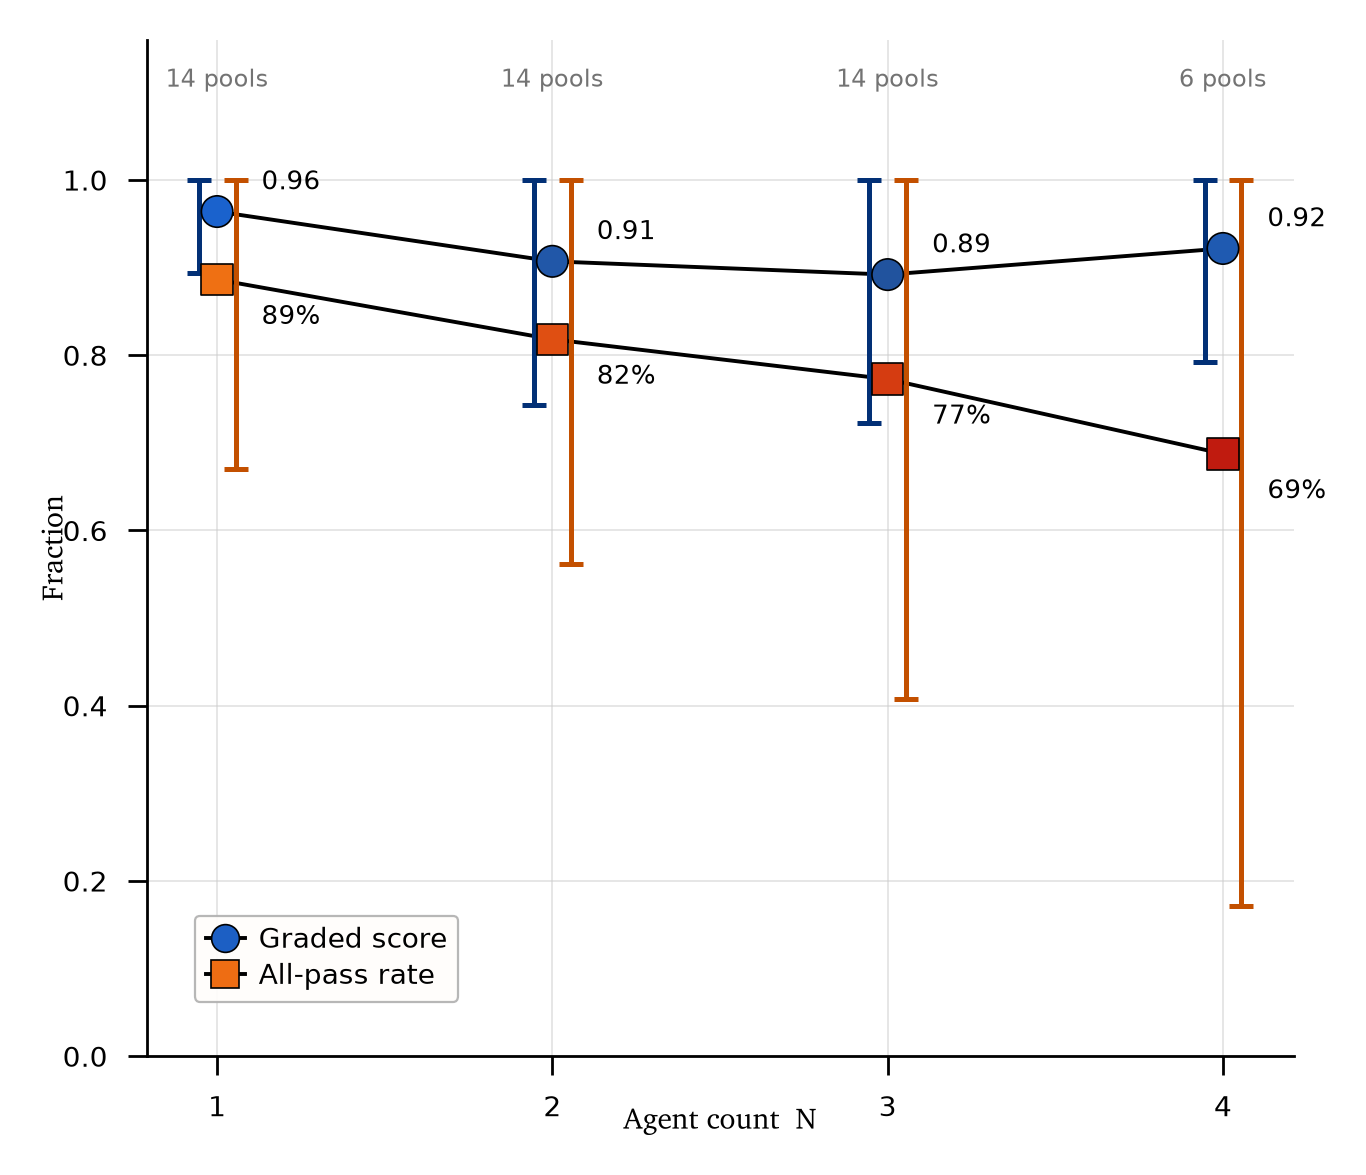
\includegraphics[width=0.6469\linewidth]{fig2a_correctness.png}
	\caption{\textbf{Adding agents buys no correctness.} The graded score (circles) holds flat while the strict all-pass rate (squares) falls 89\% $\rightarrow$ 69\%. Error bars throughout this report are 95\% confidence intervals of the mean, clustered by pool, over the pool count annotated above each point.
    }\label{fig:correctness}
\end{figure}

\FloatBarrier
\subsection{Results: Cost Rises on Every Pool}\label{sec:scalingcost}

Cost rises on every pool. It increases from \$0.78 for a solo run to \$7.21 at four agents for the same $K$ features (Figure~\ref{fig:cost}). Decomposing cost into four accounts shows redundant context ingestion grows roughly linearly (Figure~\ref{fig:decomposition}): \$0.50, \$0.92, \$1.47, \$2.27. Per-agent, work inflates super-linearly (\$0.27 to \$2.37). Each agent does more work as the team grows. Coordination adds an extra cost on top of that. The messaging channel, measured as tokens sent, received, and re-ingested, accounts for 23--25\% of every multi-agent run. Messaging also provokes rework, meaning files are re-edited in response to inbound messages. When that message-triggered rework is included, the messaging-related share rises to 31--36\% (\$0.48 communication $+$ \$0.16 rework at $N = 2$, rising to \$1.82 $+$ \$0.75 at $N = 4$).

\begin{figure}[!htb]
	\centering
	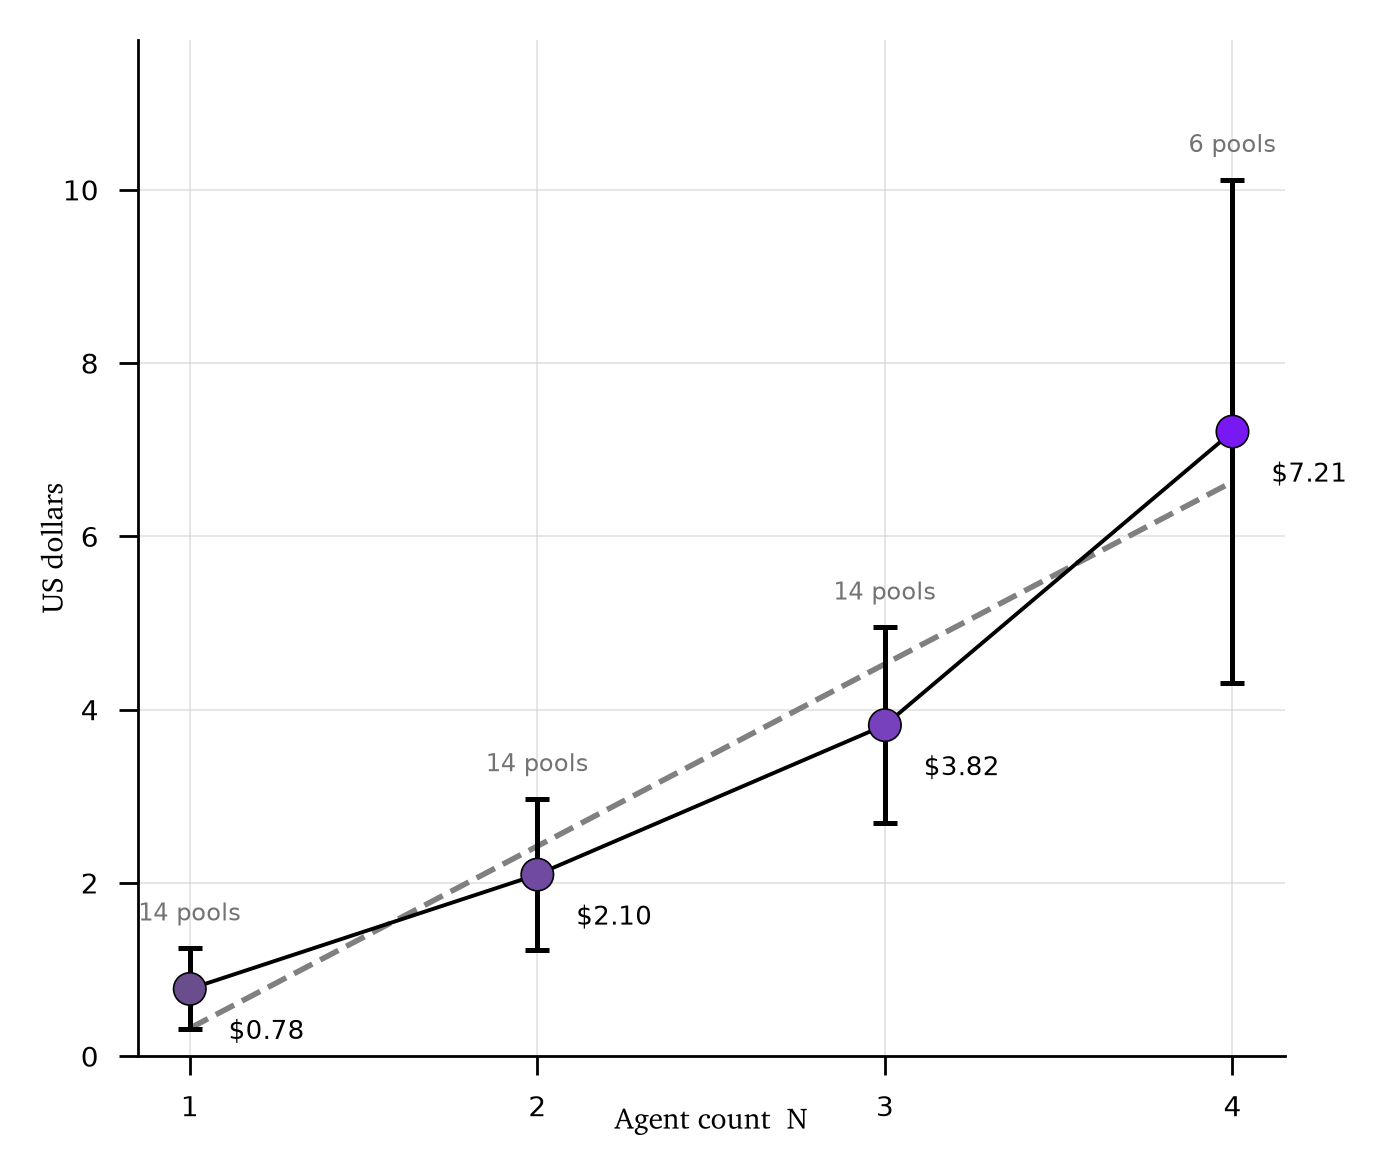
\includegraphics[width=0.6469\linewidth]{fig2b_cost.png}
	\caption{\textbf{Cost rises near-linearly in agent count.} Mean cost per run climbs \$0.78 $\rightarrow$ \$7.21, a linear trend of roughly \$2 per added agent (dashed).
    }\label{fig:cost}
\end{figure}

\begin{figure}[!htb]
	\centering
	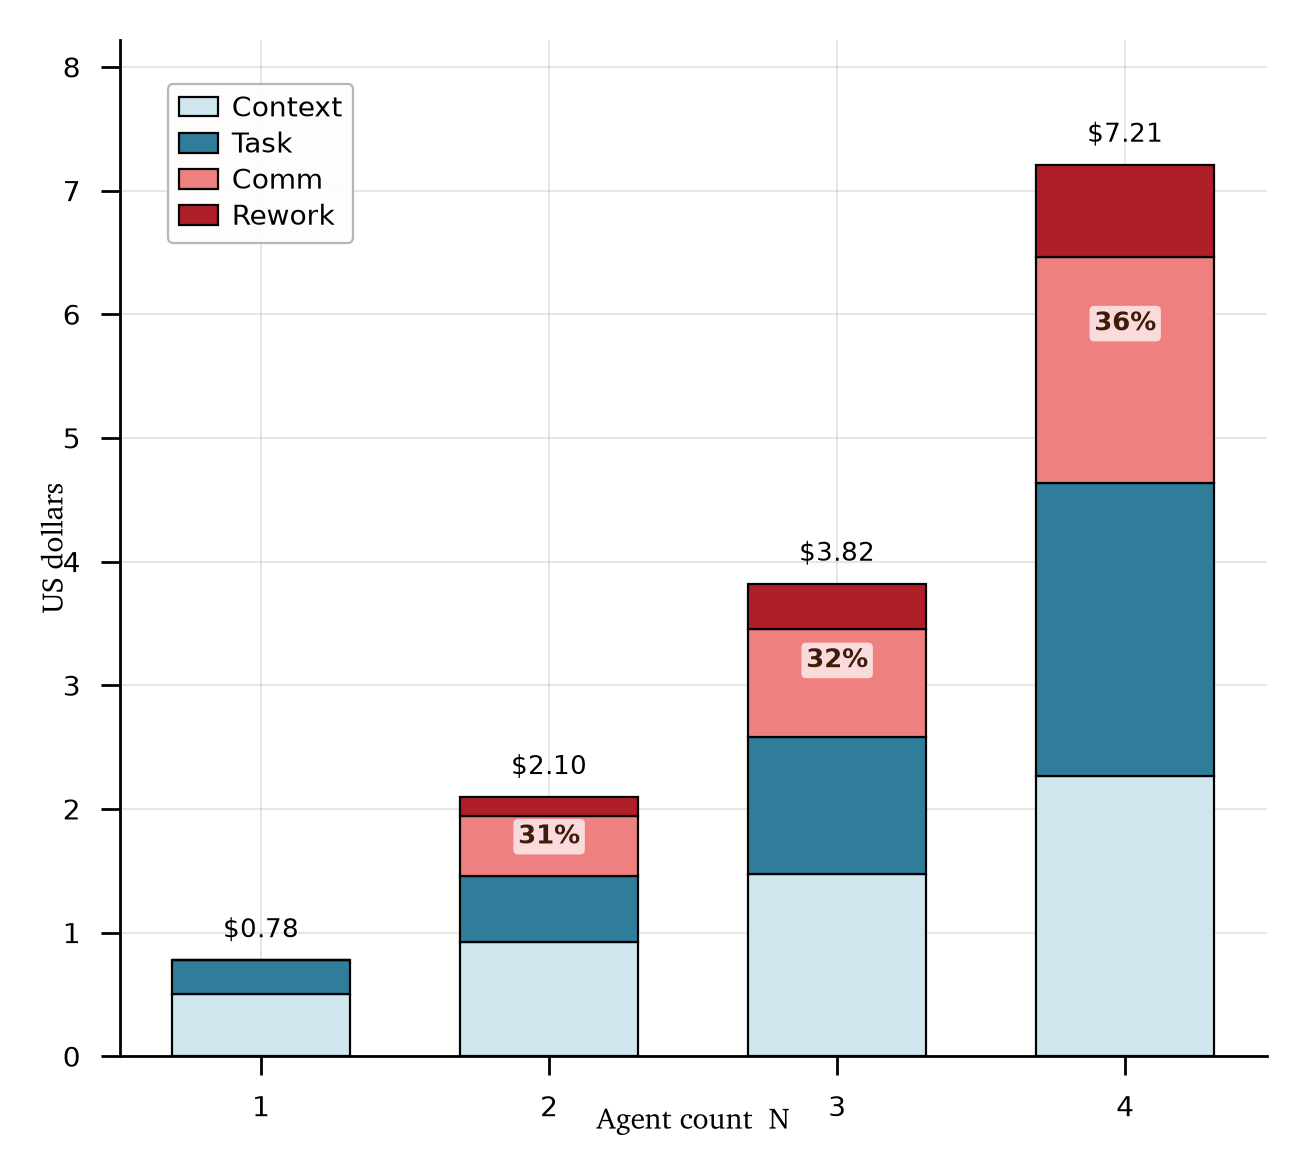
\includegraphics[width=0.6469\linewidth]{fig2d_cost_decomposition.png}
	\caption{\textbf{Decomposing the communication tax.} Per-run cost split into the four token accounts. Context is a message-independent floor; messaging and the rework it triggers are roughly a third of every multi-agent run.
    }\label{fig:decomposition}
\end{figure}

%%%%%%%%%%%%%%%%%%%%%%%%%%%%%%%%%%%%%%%%%%%%%%%%%%%%%%%%%%%%%%%%%%%%%%
%
%    A Supervisor is all They Need
%
%%%%%%%%%%%%%%%%%%%%%%%%%%%%%%%%%%%%%%%%%%%%%%%%%%%%%%%%%%%%%%%%%%%%%%
\FloatBarrier
\section{A Supervisor is all They Need}\label{sec:supervisor}

In a flat-peer topology, no single agent is responsible for governing the pool of tasks. Therefore each reconstructs the shared picture privately and then reconciles it with its peers. Making one supervisor agent responsible for the division of labour, and for the final assembly of features, replaces a decision the peers negotiate collectively with a single focused decision node.

The arrangement is not new. It is the manager--contractor structure of Smith's Contract Net Protocol~\cite{smith1980contractnet}, the seminal architecture for task allocation in distributed problem solving, in which one distinguished node decomposes a problem, announces the resulting subtasks, awards each to a contractor, and is answerable for the assembled result. Davis and Smith~\cite{davis1983negotiation} give the fuller account of why control is centralised this way: the manager holds the global view that no contractor has, so allocation is decided once rather than negotiated pairwise. What we vary here is only that --- who decides the division of labour, and who assembles the result --- while every other property of the apparatus is held at the values of Section~\ref{sec:growth}.

If the tax we have measured is based on mutual coordination, centralising it should therefore reduce it. Figure~\ref{fig:suparch} sets out the resulting arrangement.

\subsection{Methodology}\label{sec:supdesign}

\begin{figure}[!ht]
	\centering
	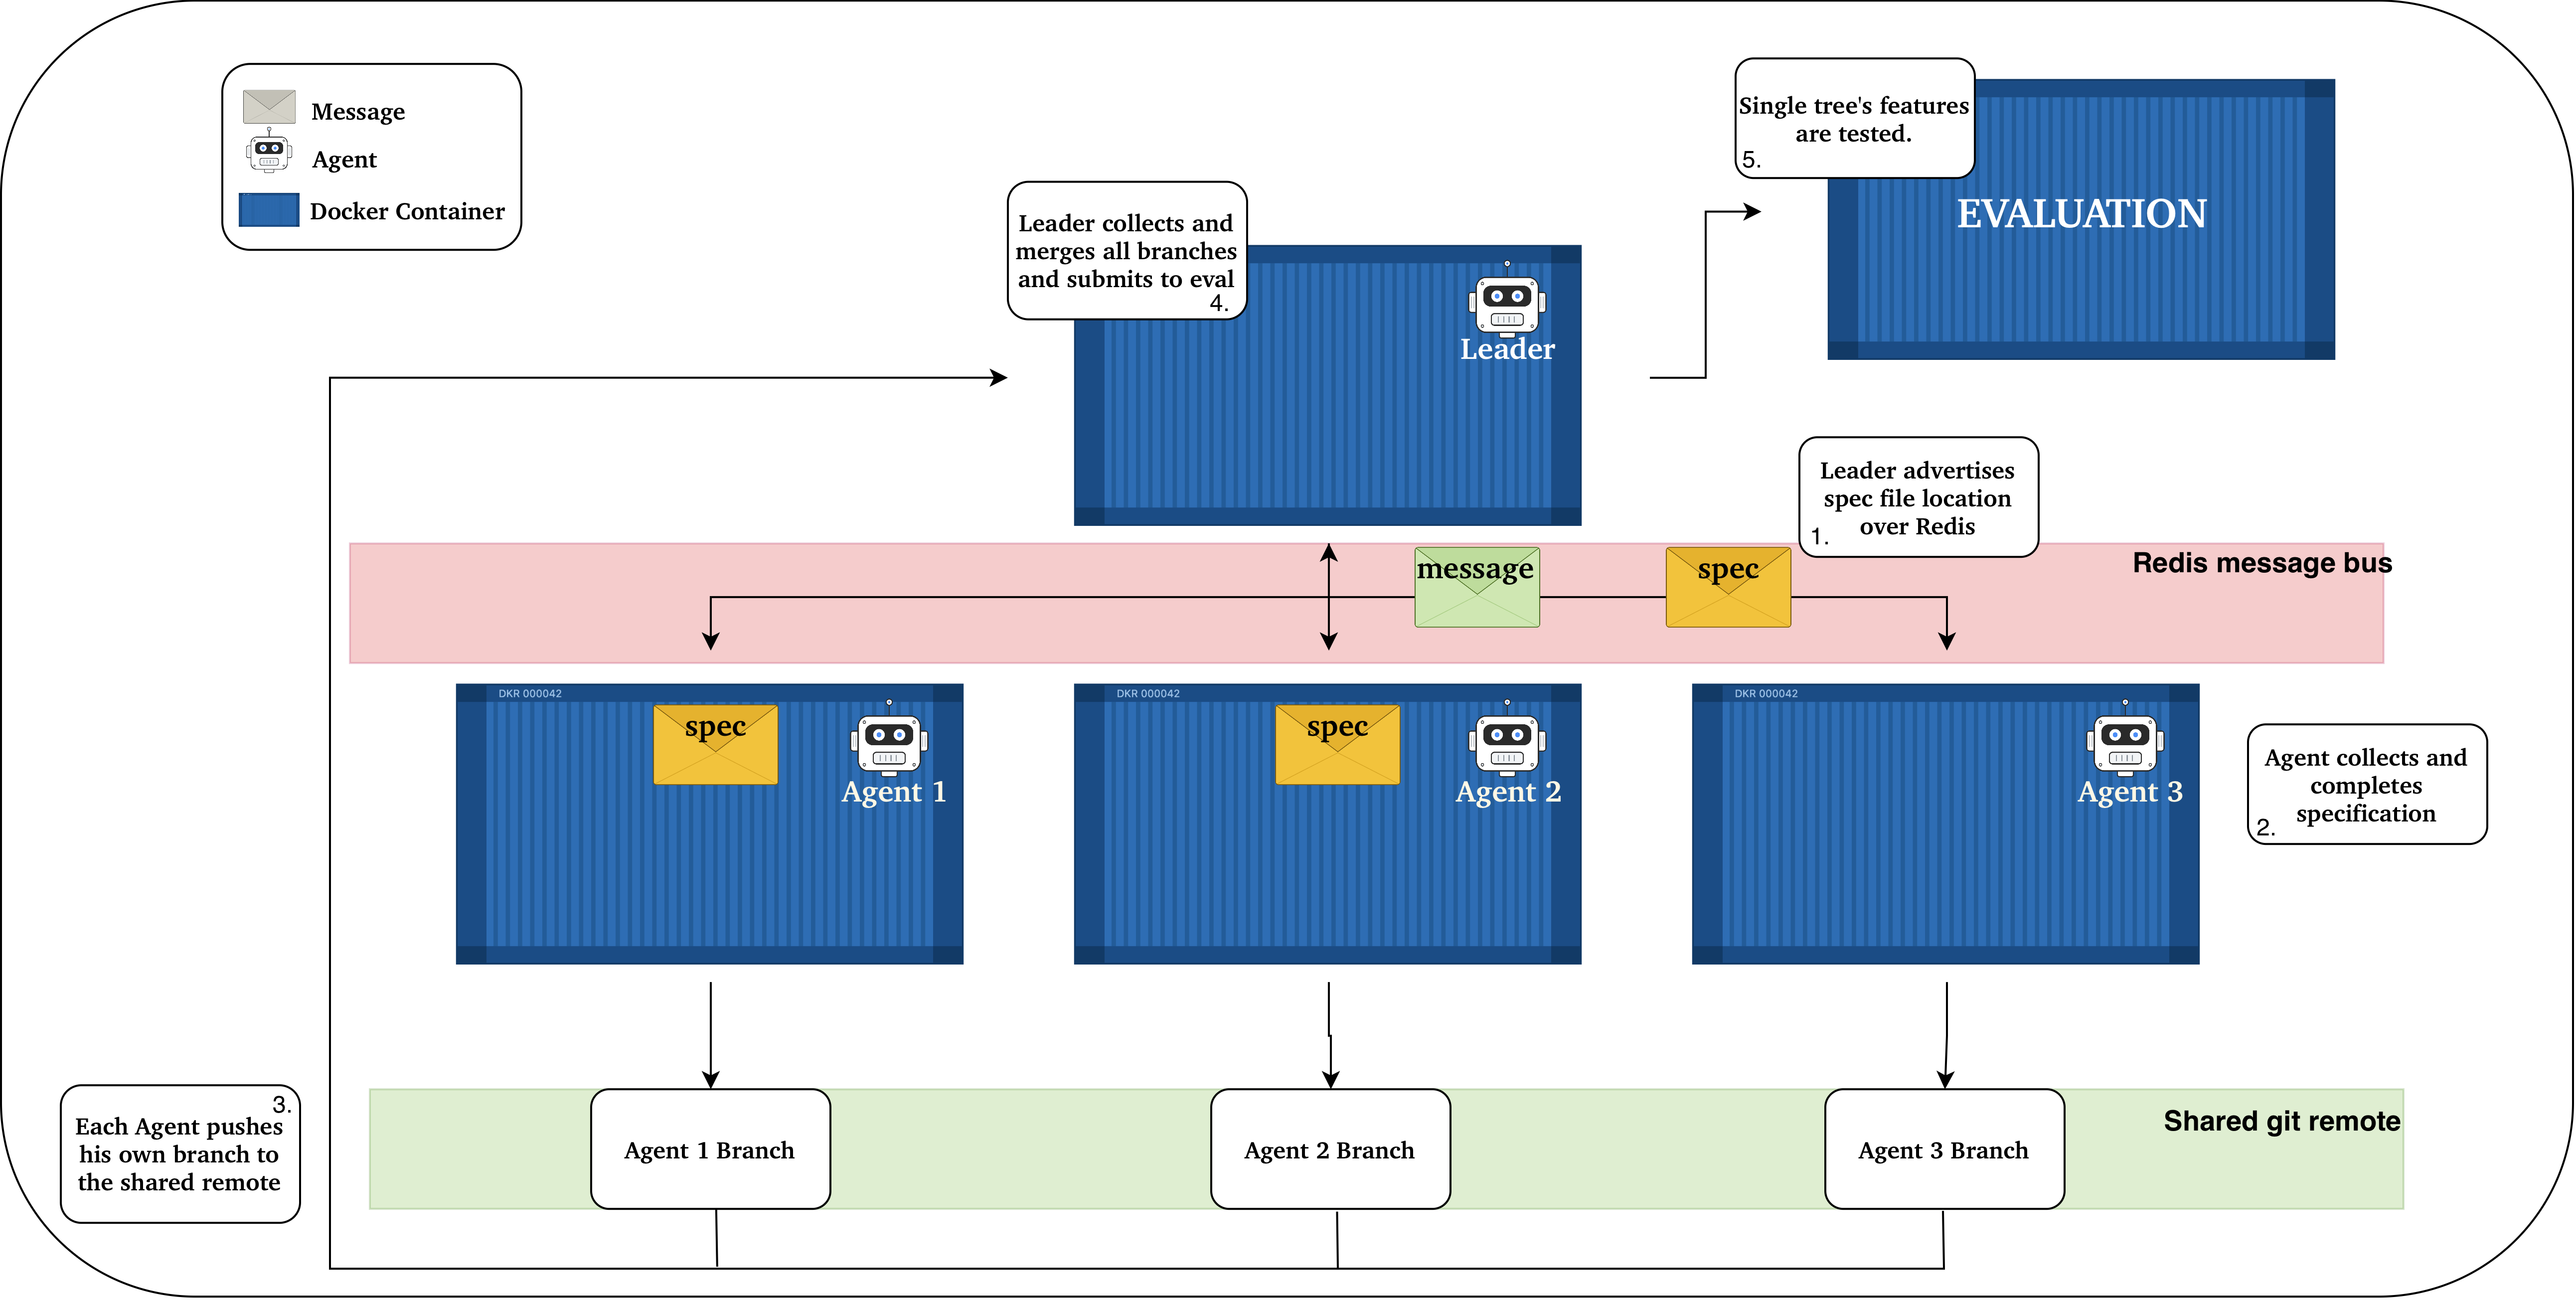
\includegraphics[width=\linewidth]{fig4_supervisor_architecture.png}
	\caption{\textbf{The supervised topology.} (1)~The leader advertises each specification over Redis; (2)~each worker implements only its own; (3)~workers push their own branch and stop, never merging a peer; (4)~the leader collects every branch, performs the team's single integration, and submits; (5)~that one tree is scored against all $K$ suites. Contrast the $N$ integrations of Figure~\ref{fig:flatarch}.
    }\label{fig:suparch}
\vspace{0.8\baselineskip}
\end{figure}

The apparatus, workload, and evaluation are held fixed at the values used in Section~\ref{sec:growth}: the same 14 pools, shared git remote and the same graded scoring of one integrated tree against all $K$ test suites.

The only change is the topology. In the supervised arm, a leader agent (Claude Sonnet 5) is the only participant that receives the $K$ feature specifications. It writes a decomposition plan. It materialises each specification into a shared scratchpad and assigns features to workers (Claude Sonnet 5) through a shared task list. It monitors progress and is the designated integrator whose tree the evaluation scores. Worker agents begin with no specification at all. Instead, they are instructed to poll the shared task list, claim their assigned-task location and collect it. They are instructed to implement only what they are assigned. The round-robin partition --- a fixed, benchmark-imposed allocation in the flat arm --- is thus replaced by an allocation the leader chooses. Integration is also centralised. Workers are instructed to commit their own feature, push their own branch and exit. Finally, the supervisor is instructed to assemble the team's single tree and submit it for evaluation. The Redis messaging channel does not change. Workers are still able to communicate freely between other workers. They are never, however, instructed to do so. Every isolated container receives a roster of the addresses of the other participants. The hierarchy is therefore a property of the agents' system prompt, not infrastructure --- this allows us to consider \emph{only} a change in topology in an attempt to remove all other aspects of variability. In practice, workers do not message other workers. Across the 144 runs, the agents exchanged 384 messages, of which 286 (74.5\%) ran supervisor-to-worker and 97 (25.3\%) worker-to-supervisor. The supervisor is considered an additional agent: comparisons are therefore made at $A = N$ (flat peers) versus $A = N + 1$ (supervised) at matched $A$, where $N$ is the number of workers. A flat-peers run of 3 agents is comparable to a single supervisor and $N = 2$ worker agents. The dataset is 144 total runs (${\sim}\$446$ API-equivalent) --- $r = 3$ trials over 48 cells (14 pools $\times$ $N \in \{1, 2, 3\}$, plus the six $K = 4$ pools at $N = 4$).

\subsection{Cost}\label{sec:supcost}

Matched pool-for-pool --- comparing only the pools both arms ran, so the mix of easy and hard workloads is identical on each side --- the supervisor topology costs $1.05\times$ flat peers at two agents, $0.72\times$ at three and $0.51\times$ at four. Efficiency --- work solved per dollar --- follows: $0.93\times$, $1.38\times$ and $1.81\times$ (Table~\ref{tab:topology}). The gap has a single mechanism: a flat team pays its coordination once per agent --- every peer merges every other and messages every other, so the bill grows with each agent added --- while the supervised team pays it once in total, one integration and one hub of messages, leaving little in a supervised run's cost to grow beyond the workers themselves.

\begin{table}[h!]
\centering
\vspace{0.9\baselineskip}
	\caption{Flat-peer and supervised topologies by total agent count $N$, averaged over all pools (144 supervised runs, 148 flat).\label{tab:topology}}
   \renewcommand{\arraystretch}{1.1}
   \setlength{\tabcolsep}{5pt}
\begin{tabular}{ccccccc}
 \toprule
 & \multicolumn{3}{c}{Flat peers} & \multicolumn{3}{c}{Supervised} \\
 \cmidrule(lr){2-4} \cmidrule(lr){5-7}
 $N$ & Score & Cost & Solved per \$ & Score & Cost & Solved per \$ \\
 \midrule
 1 & 0.96 & \$0.78 & 1.24 & --- & --- & --- \\
 2 & 0.91 & \$2.10 & 0.43 & 0.88 & \$2.37 & 0.37 \\
 3 & 0.89 & \$3.82 & 0.23 & 0.90 & \$2.93 & 0.31 \\
 4 & 0.92 & \$7.21 & 0.13 & 0.90 & \$3.20 & 0.28 \\
 5 & --- & --- & --- & 0.92 & \$4.95 & 0.19 \\
 \bottomrule
\end{tabular}
\vspace{0.9\baselineskip}
\end{table}

The efficiency collapses as a power law again --- efficiency $= 0.63 \cdot N^{-0.69}$. Recall flat peers --- efficiency $= 1.28 \cdot N^{-1.61}$ (Figure~\ref{fig:topoeff}). For a fixed workload divided among $N$ agents, one would expect efficiency to fall as $1/N$, where we pay for $N$ agents to do a pool of work. $b = 1$ is therefore the reference, the value at which coordination itself costs nothing extra. Supervision's $b = 0.69$ sits comfortably below that reference. As the team grows, each worker implements fewer features while the supervisor's overhead is amortised over more of them, so total cost grows sublinearly in $N$.

\begin{figure}[!htb]
	\centering
	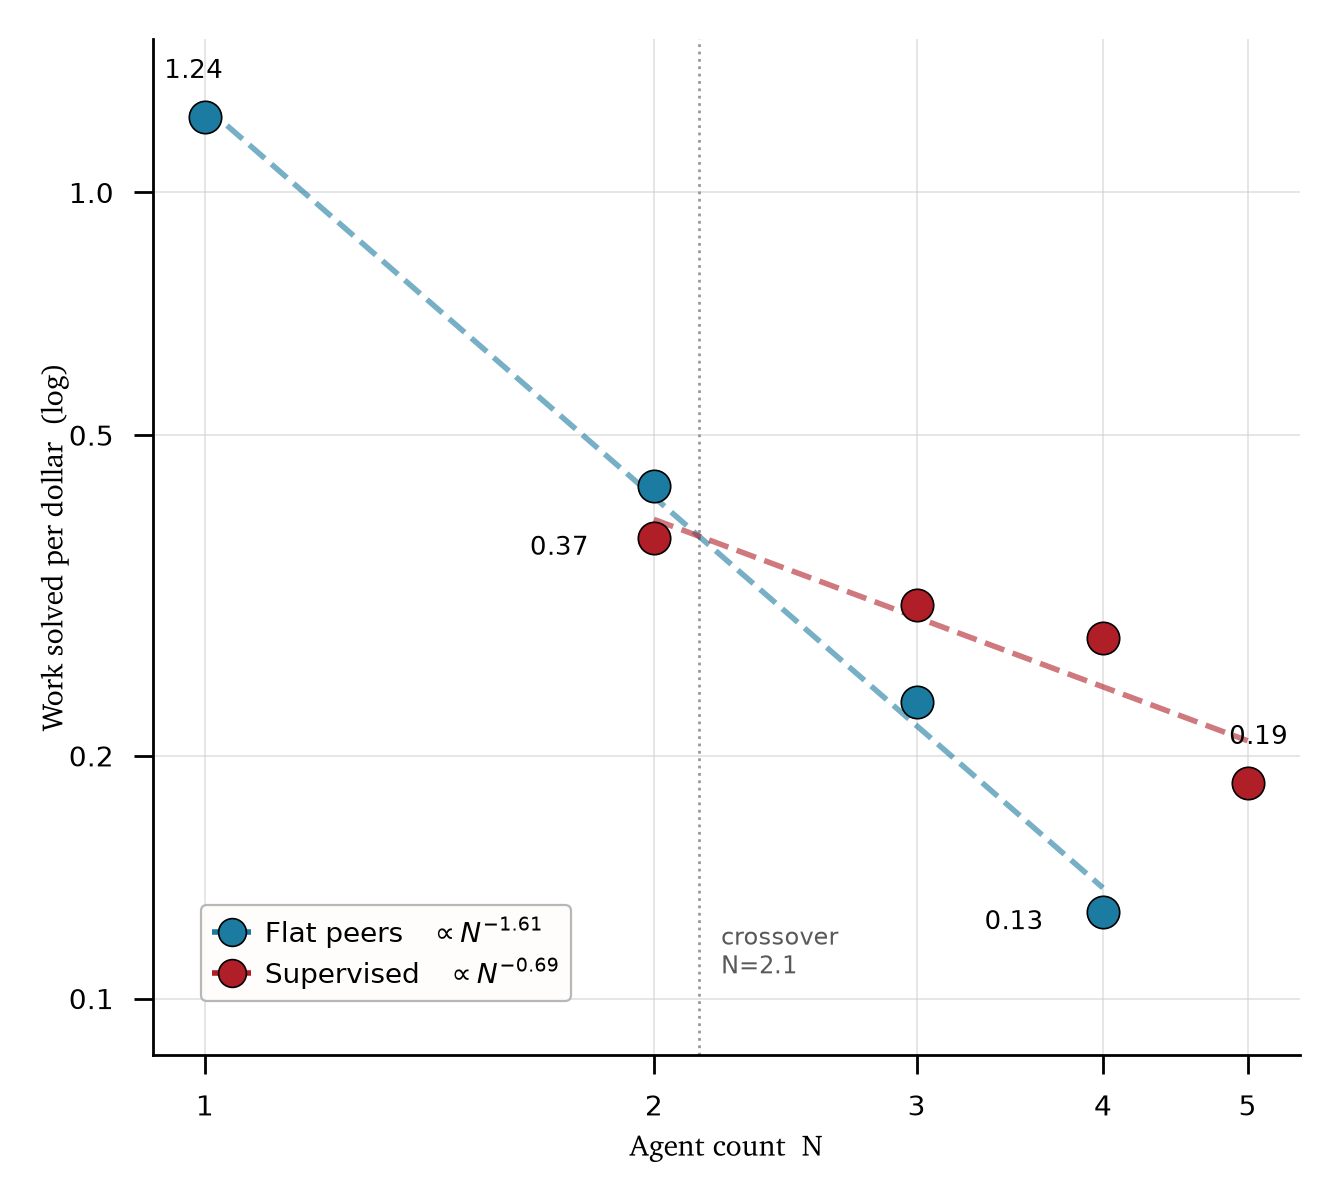
\includegraphics[width=0.6469\linewidth]{fig3a_efficiency_topology.png}
	\caption{\textbf{Efficiency by topology (log--log).} Fitted power laws $1.28 \cdot N^{-1.61}$ flat and $0.63 \cdot N^{-0.69}$ supervised; the dotted vertical marks the crossover at $N \approx 2.1$.
    }\label{fig:topoeff}
\end{figure}

\begin{figure}[!htb]
	\centering
	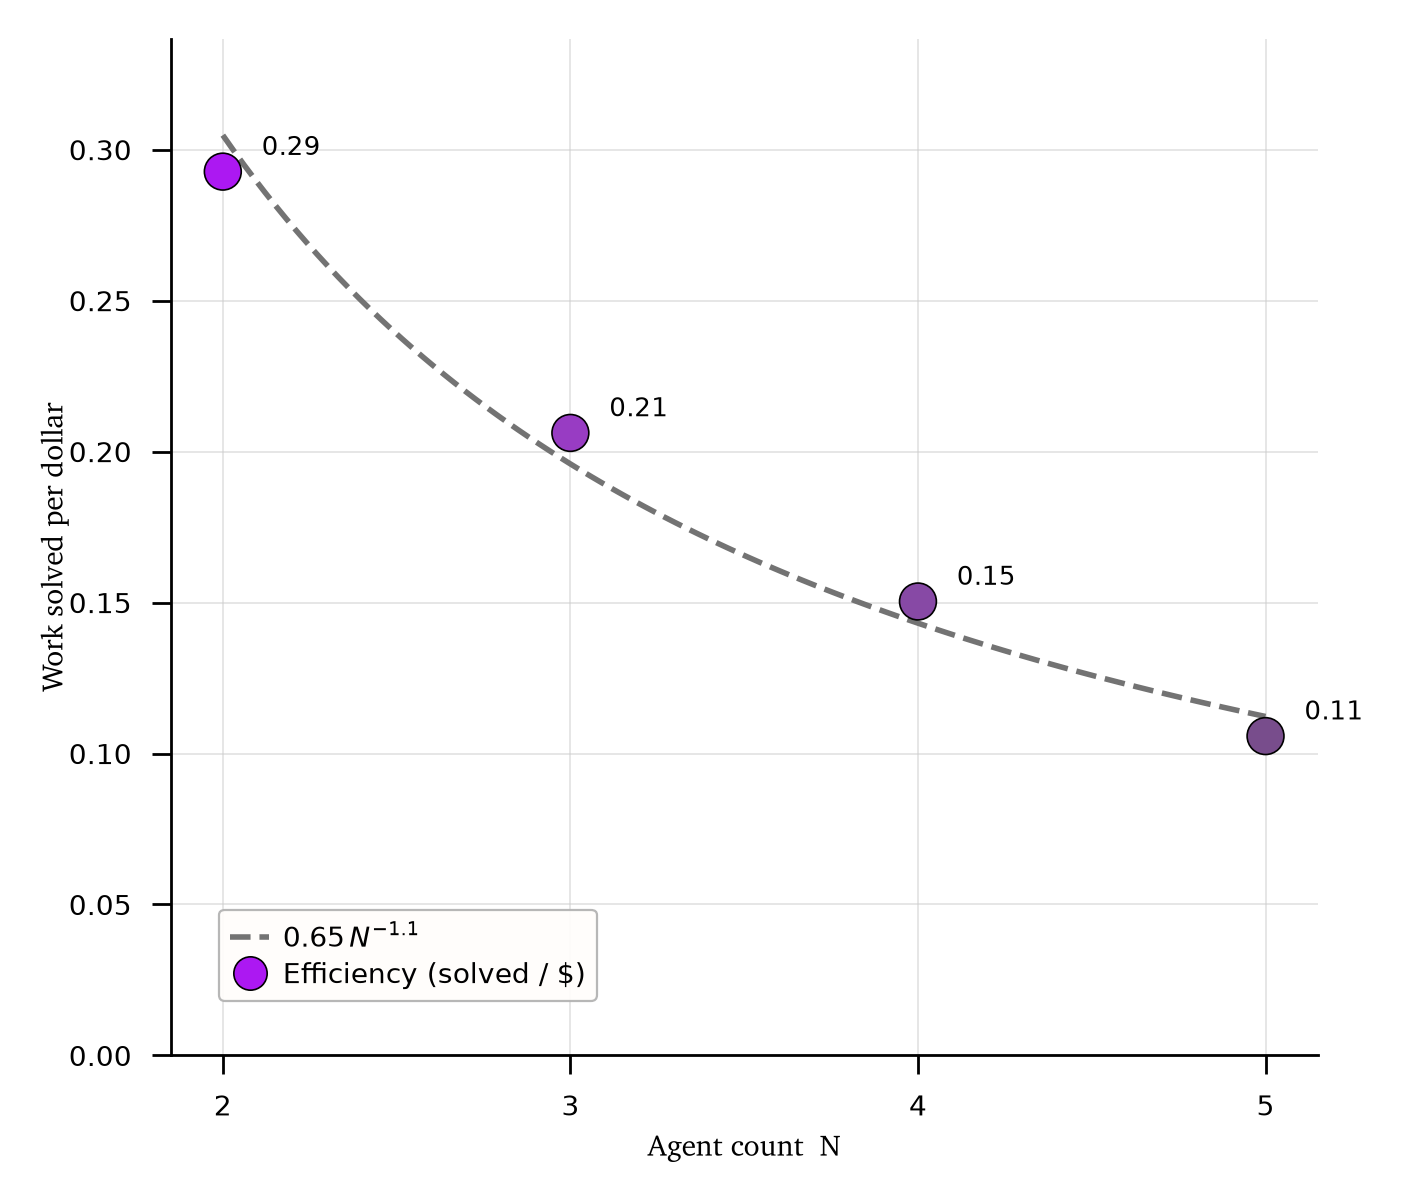
\includegraphics[width=0.6469\linewidth]{fig3e_efficiency_supervised.png}
	\caption{\textbf{The supervised arm's efficiency decline.} 0.37 $\rightarrow$ 0.19 solved per dollar across 2--5 agents --- far shallower than the flat arm's collapse (Figure~\ref{fig:efficiency}).
    }\label{fig:supeff}
\end{figure}

The cost accounts locate the mechanism (Figure~\ref{fig:topoaccounts}). The communication and rework accounts together are 5.4\%, 10.1\%, 8.3\% and 15.4\% of the supervised run across two to five agents, versus 30.6\%, 32.5\% and 35.7\% of the flat peer-to-peer arm at two to four agents. Taken together, the three views say the same thing: under flat peers, coordination is a cost that compounds --- a super-proportional exponent fed by a messaging share that grows toward a third of every run --- while under supervision it behaves almost as a fixed fee, paid once and amortised as workers are added. From three agents upward, hierarchy is simply the cheaper way to divide the same work. Neither topology, however, reduces the context floor beneath both, which is why no team of any shape beats the solo agent.

\begin{figure}[!htb]
	\centering
	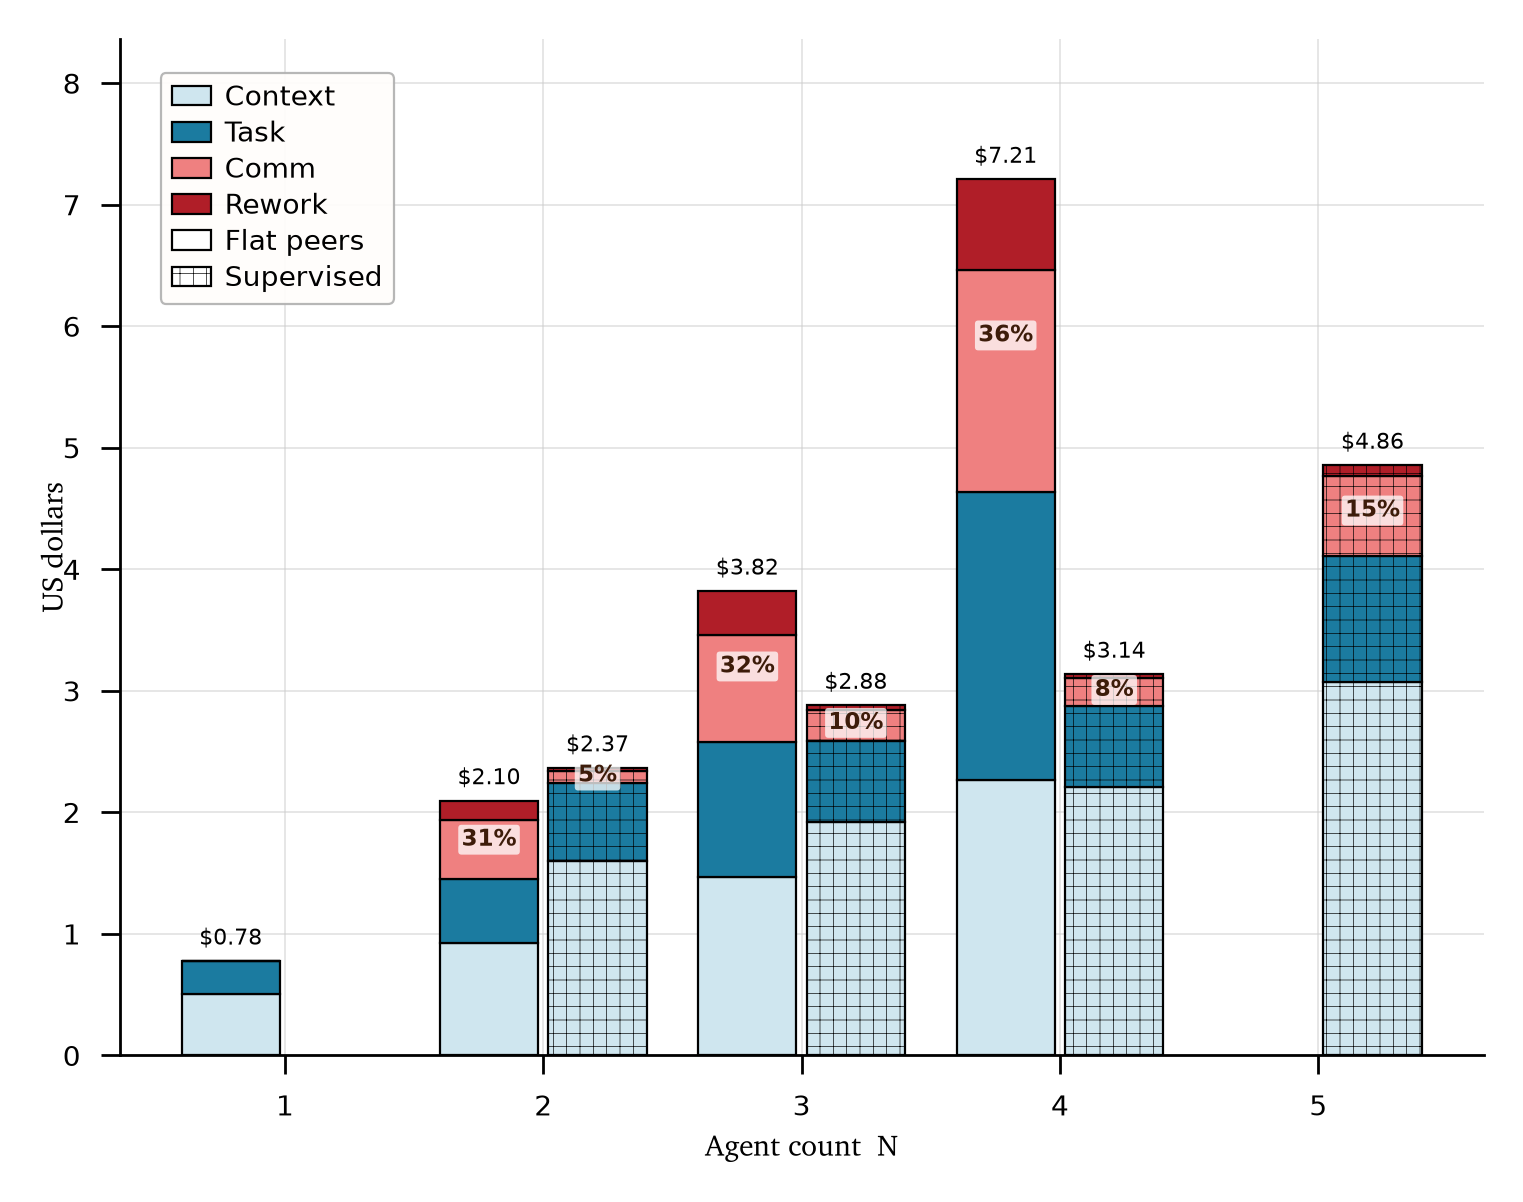
\includegraphics[width=0.6469\linewidth]{fig3c_accounts_topology.png}
	\caption{\textbf{Cost accounts by topology.} Flat peers are the solid left bar of each pair, supervised the cross-hatched right. The warm cap is comm $+$ rework as a share of the run: 5--15\% supervised against 31--36\% flat.
    }\label{fig:topoaccounts}
\end{figure}

\subsection{Correctness}\label{sec:supcorrect}

On correctness, the two topologies diverge. Under the supervision topology, the graded score (number of test suites passed / total features) is 0.883, 0.903, 0.895 and 0.917 across two to five agents. Recall the flat peer-to-peer 0.907, 0.892, 0.922. On the strict all-pass rate, the supervised arm runs 79\%, 81\%, 76\% and 83\%. Recall the flat peer-to-peers' monotone decline of 89\%, 82\%, 77\%, 69\% from one to four agents (Figure~\ref{fig:topocorrect}). Therefore, at four agents, supervision is ahead on the strict all-pass rate (76\% versus 69\%) and behind on the graded score (0.895 versus 0.922). The key takeaway here is that supervision maintains the correctness whereas flat peers reduce it as the team scales. The flat peer-to-peer arm loses 20 points of all-pass rate across its range whereas the supervised arm ends where it began. Neither arm approaches the solo baseline value of 0.964 and 89\%.

\begin{figure}[!htb]
	\centering
	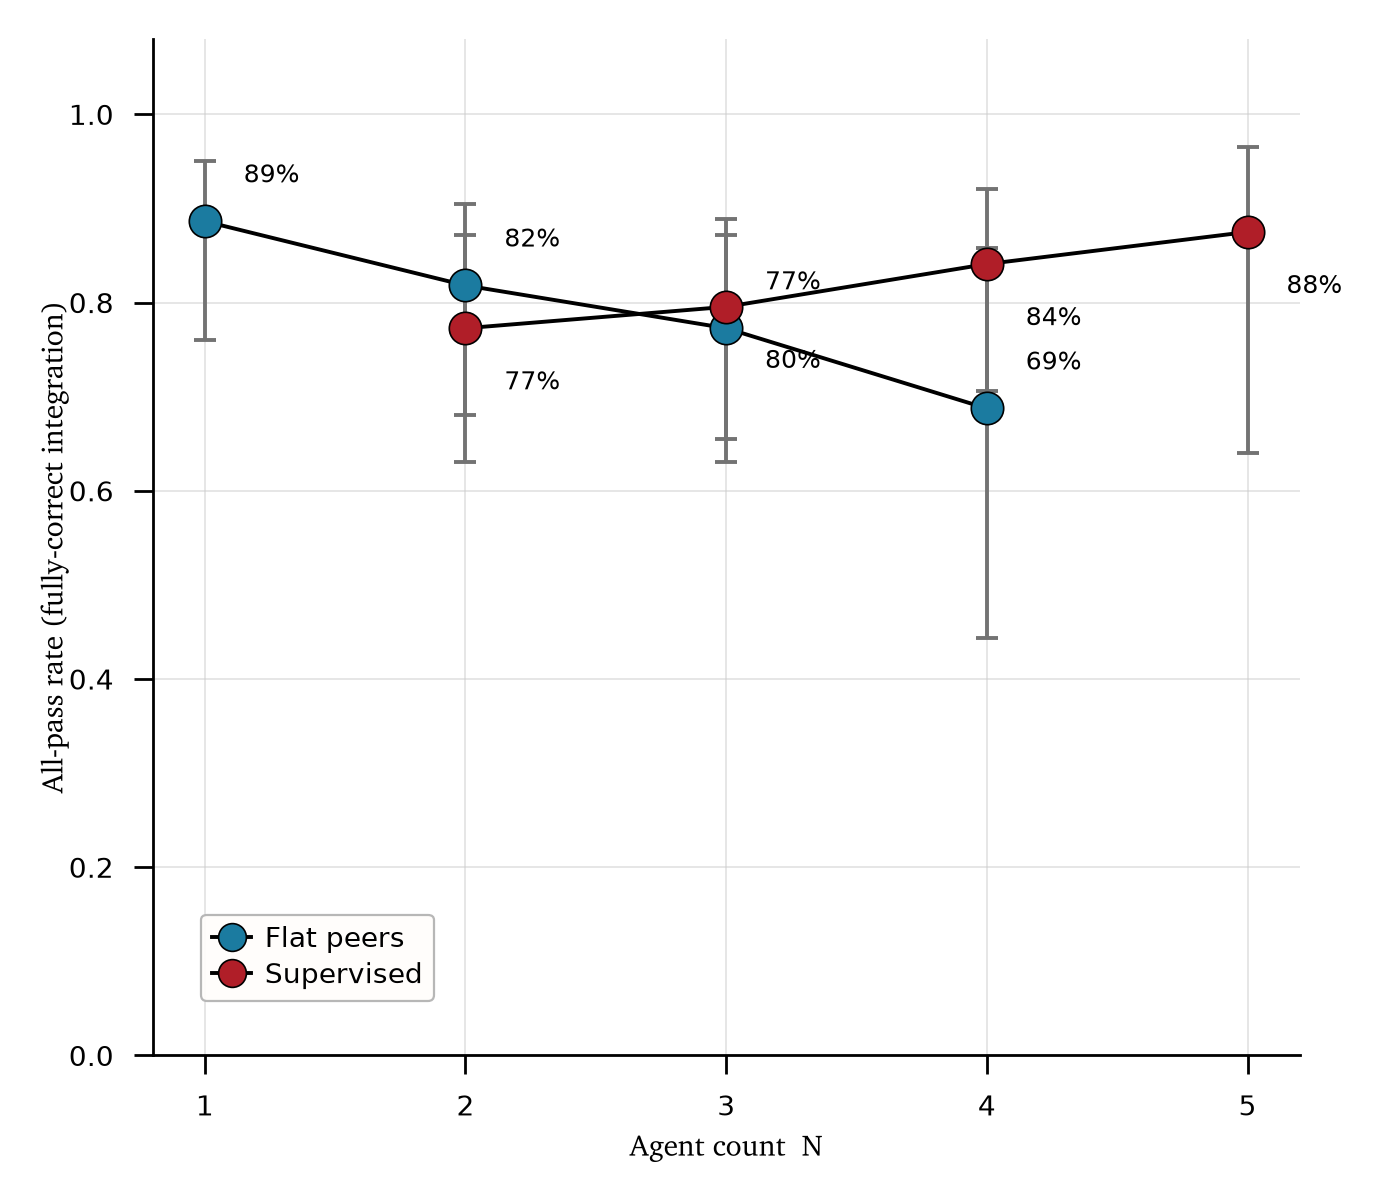
\includegraphics[width=0.6469\linewidth]{fig3b_correctness_topology.png}
	\caption{\textbf{Correctness holds under supervision and falls under flat peers.} Strict all-pass rate: flat peers fall 89\% $\rightarrow$ 69\%, supervision stays between 76\% and 83\%.
    }\label{fig:topocorrect}
\end{figure}

The data distribution can explain why the two arms diverge. The flat peers fail monotonically and increasingly. The share of partial success grows 11\%, 14\%, 21\%, 31\% from one to four agents. Supervision, on the other hand, holds its share of partial successes (14\%, 14\%, 19\%, 11\% across two to five). It carries a consistent floor of total failures (7\%, 5\%, 5\%, 6\%). Centralising integration therefore makes the supervisor a single point of success. If its merge lands, everything lands, and if it fails, everything is lost. No partial contribution survives.

\FloatBarrier
\subsection{What This Shows}\label{sec:supshows}

Hierarchy is not a cure for the communication tax, but it is a substantially better trade-off than flat peers once a team exceeds two agents. Centralising both allocation of features and the integration of code cuts the messaging-related share of a run from roughly a third to under a sixth. It also flattens the efficiency exponent from $N^{-1.61}$ to $N^{-0.69}$. It holds correctness where flat peers degrade. Albeit at the cost of converting some partial successes into total failure, it still, however, is not favoured over a single model instance. The solo agent remains better than every configuration of every topology measured here, scoring 0.964 at \$0.78. No supervised cell comes within a factor of three of the solo efficiency.

%%%%%%%%%%%%%%%%%%%%%%%%%%%%%%%%%%%%%%%%%%%%%%%%%%%%%%%%%%%%%%%%%%%%%%
%
%    Wall-Clock Time (flat peers and supervision)
%
%%%%%%%%%%%%%%%%%%%%%%%%%%%%%%%%%%%%%%%%%%%%%%%%%%%%%%%%%%%%%%%%%%%%%%
\FloatBarrier
\section{Wall-Clock Time: Sharing the Work Does Not Make It Faster}\label{sec:wallclock}

One of the main benefits of sharing work is the potential for decreased wall-clock time. Sharing work across more workers should theoretically reduce the total time spent working. A system that has to sequentially run tasks will take longer than one that can run the tasks in parallel. A perfect parallel execution would therefore present itself as $T_1/N$, where $T$ is the time to completion and $N$ is the number of agents. This uses data collected from the flat-peers study as well as the supervisor study --- 148 flat-peer runs and 144 supervised runs. No new apparatus is required. A run's wall-clock time is calculated when the final agent stops.

\begin{figure}[!htb]
	\centering
	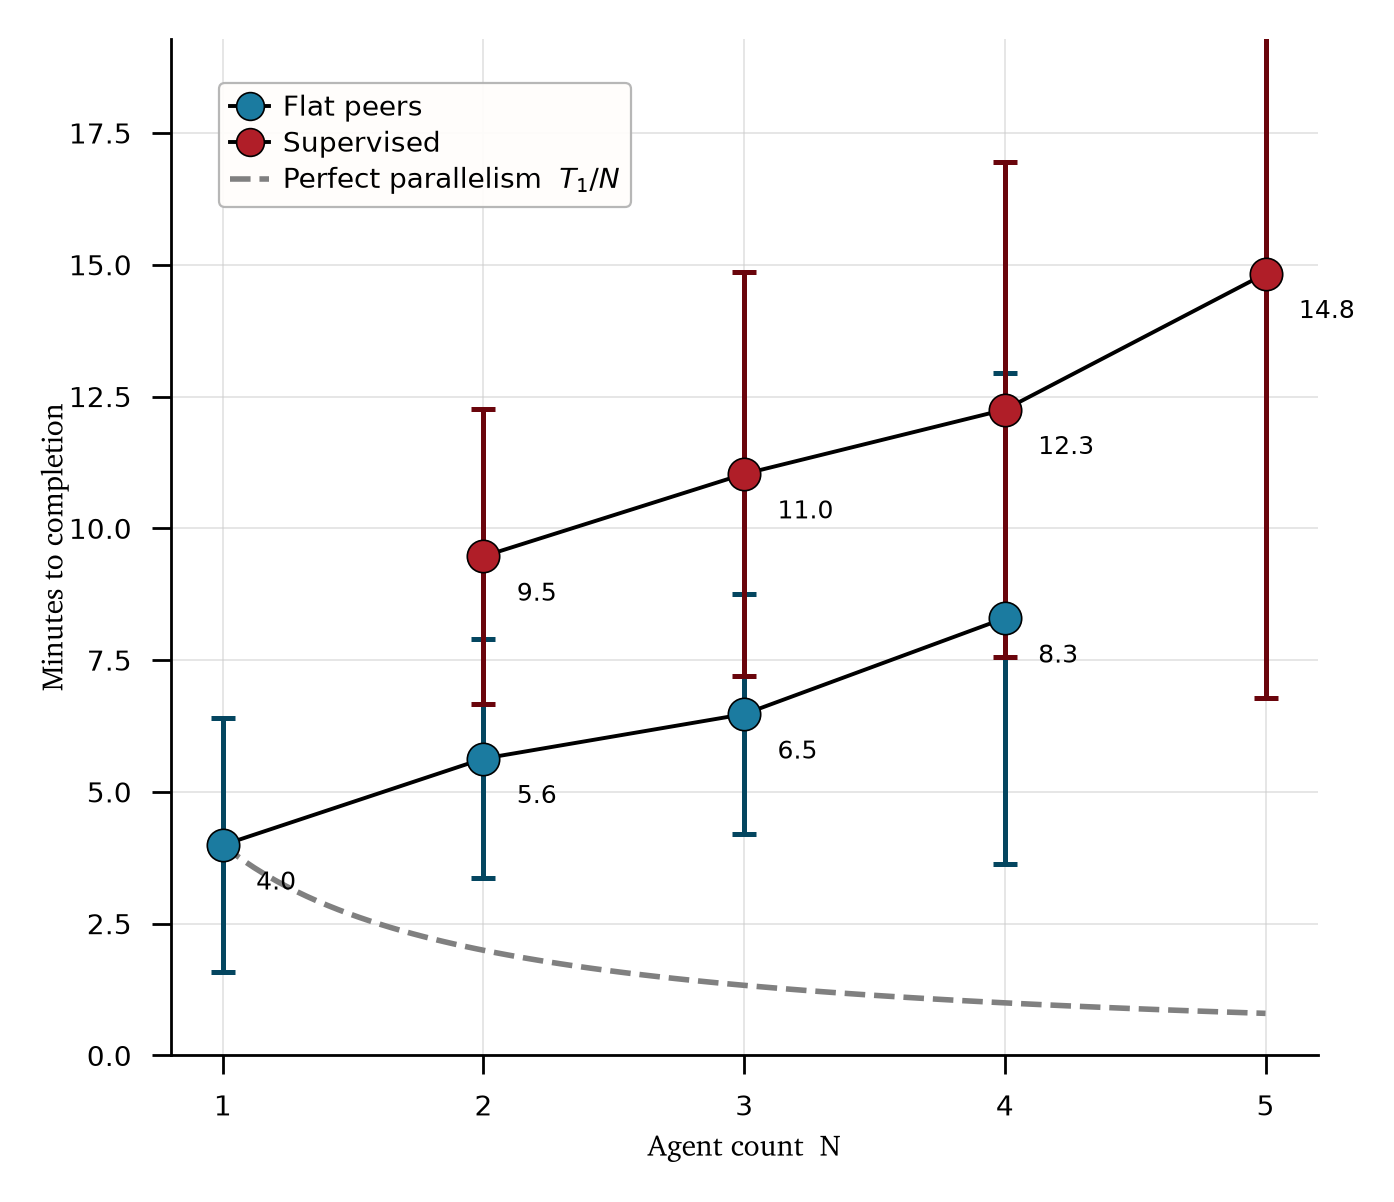
\includegraphics[width=0.6469\linewidth]{fig3d_wallclock_topology.png}
	\caption{\textbf{Hierarchy is slower still, but converging.} Supervision runs 7.3 $\rightarrow$ 11.1 minutes across 2--5 agents against the flat arm's 5.6 $\rightarrow$ 8.3, the gap narrowing as teams grow.
    }\label{fig:topowall}
\end{figure}

\FloatBarrier
\subsection{Flat Peers}\label{sec:wallflat}

Flat peers do not deliver the $T_1/N$ parallelism. A solo agent completes the full $K$-feature pool in 4.0 minutes on average; two agents take 5.6, three take 6.5, and four take 8.3. Wall-clock time therefore rises with team size. Coordination lengthens the overall time an agent spends completing their work. They must spend time reading replies, waiting on replies, writing and sending messages. We suspect, however, that this inversion is likely an artifact of scale. Increasing the time spent solving features could see a different result. At the current small scale, agents spend a considerable amount of time messaging. For larger individual tasks, where a greater proportion of time is spent implementing the feature, a genuine wall-clock speedup could emerge. Locating the task size at which parallelism starts to pay is a natural target for future work.

\subsection{Hierarchy}\label{sec:wallhier}

A supervised team is slower than a flat-peers team at every size: 7.3 versus 5.6 minutes at two agents, 8.2 versus 6.5 at three agents, and 8.8 versus 8.3 at four agents. The gap, however, closes as the team scales --- supervision is 30\% slower at two agents but only 6\% at four (Figure~\ref{fig:topowall}).

Both topologies still remain slower than their solo counterpart. The supervised arm realises $0.52\times$ speed at two agents compared to solo, falling to $0.43\times$ speed at five. The flat arm realises a slightly improved $0.66\times$ speed at two agents and a $0.56\times$ speed at four.

The reason is the shape of a supervised run, which is like book-ends: a serial opening, a parallel middle, and a serial close --- with the supervisor alone on the clock at both ends. In all 144 runs the supervisor finished last. The opening is allocation: every worker sits idle while the supervisor reads the $K$ specifications, writes the plan, and creates the tasks, taking 2.7 minutes at one worker and 3.2 at four. The close is integration: the supervisor merging alone after the last worker has stopped, taking 2.5 minutes rising to 4.3. The two serial segments sum to 5.3--7.5 minutes --- 65--73\% of the entire run, and on their own already as long as a complete flat-arm run. The middle, by contrast, is genuinely parallel: summed agent time grows from 12.0 to 33.5 minutes across two to five agents while wall-clock grows only from 7.3 to 11.1, so on average 1.65 to 3.03 agents are working at once. Adding workers therefore shrinks only the middle between the book-ends; the serial ends barely move, and they are most of the run.

Flat peers pay the same coordination in the opposite currency. Each peer receives its specification in its opening prompt, so no one starts idle; and each merges its peers concurrently, so integration --- performed $N$ redundant times --- runs on $N$ clocks at once rather than extending the critical path. That is cheap in time and ruinous in dollars; the supervised arm is the reverse. The flat arm's finding survives the change of topology --- sharing the work does not make it faster --- but where the flat arm's time penalty grows with the team, the supervisor's shrinks, so the two topologies converge as teams grow.

\subsection{What This Shows}\label{sec:wallshows}

Parallelism is the one benefit a team ought to deliver for free, and neither topology delivers it. Take the solo agent's speed as 1.0. Flat peers manage $0.66\times$ that speed at two agents, falling to $0.56\times$ at four. Supervision is slower still: $0.52\times$ at two agents, down to $0.43\times$ at five. Every one of those numbers is below one, and adding agents never buys them back. A team here is not an imperfect parallel machine but a slower serial one. The division of labour is real; the coordination laid on top of it simply eats more clock than the division saves. One caveat bounds both arms equally. A solo agent completes the entire pool in 4.0 minutes on average, so coordination takes up a large share of every run and swamps whatever the split saves. A longer task would leave more room for parallelism to pay for itself. How much longer, these pools cannot say.

%%%%%%%%%%%%%%%%%%%%%%%%%%%%%%%%%%%%%%%%%%%%%%%%%%%%%%%%%%%%%%%%%%%%%%
%
%    Conclusion
%
%%%%%%%%%%%%%%%%%%%%%%%%%%%%%%%%%%%%%%%%%%%%%%%%%%%%%%%%%%%%%%%%%%%%%%
\FloatBarrier
\section{Conclusion}\label{sec:conclusion}

This work asked whether the coordination gap between LLM coding agents is an artifact of benchmark design or a systematic cost of dividing work a single agent can already do. Four results answer it.

First, the gap replicates under a stronger, paired design. On 46 matched feature pairs with an identical model, the solo pass rate of 44.2\% fell to 12.3\% under free-text messaging (Wilcoxon $W = 2.5$, $p < .001$). Per-feature evaluation localises the loss: paired agents pass their own feature's held-out suite as often as solo agents (21/47 vs 20/47), so pairing costs nothing in individual capability. Of the 20 pairs demonstrably solvable by one agent, cooperating pairs delivered only 5, and every loss was a textual merge conflict rather than a functional incompatibility. The coordination gap is, on this data, an integration gap.

Second, the gap widens once computational effort is normalised: 0.675 passes per dollar solo against 0.107 under messaging ($p < .001$) --- a 6.3-fold efficiency penalty against the 3.6-fold gap in raw pass rate. Coordination does not merely lower success; it makes each success more expensive.

Third, the scaling study shows the penalty compounds with team size. Holding a solo-achievable workload of $K$ mutually conflicting features fixed while varying only $N \in \{1, 2, 3, 4\}$, with integration performed by the agents themselves, adding agents bought no correctness --- the strict all-pass rate fell monotonically from 89\% to 69\% --- while cost rose near-linearly (mean $\approx \$2.04$ per added agent). Efficiency therefore collapses as a power law, $\approx 1.28 \cdot N^{-1.61}$ ($R^2 = 0.996$), with all fourteen pools individually fitting exponents between 1.1 and 2.3; at four agents, work delivered per dollar is ${\sim}10\%$ of the solo value. Because the exponent exceeds 1 everywhere --- including on pools that integrate perfectly at every $N$ --- the penalty cannot be attributed to coordination \emph{failure}. It is the price of coordination itself: a structural floor of redundant context loading, paid before any message is sent, beneath the stacked overhead of task, messaging, and rework --- the last two of which account for roughly a third of every multi-agent run.

Fourth, topology reshapes the tax without removing it. Replacing flat peers with a supervisor--worker hierarchy --- a supervisor that plans the decomposition, allocates features to workers, and performs the team's single integration --- is marginally more expensive at two agents and slower at every size, and it converts some graceful partial degradation into total failure. What it buys is the exponent: supervised efficiency falls as $0.63 \cdot N^{-0.69}$ ($R^2 = 0.856$) against the flat arm's $1.28 \cdot N^{-1.61}$ ($R^2 = 0.996$), so the curves cross at ${\approx}2.1$ agents and supervision is cheaper on 13 of 14 pools at three agents and all six at four. On strict correctness supervision holds between 76\% and 83\% across two to five agents while flat peers fall monotonically 89\% $\rightarrow$ 69\%. The mechanism is centralisation, and one half of it is adopted rather than imposed: the same fully connected channel is available in both arms, yet every supervised message passes through the supervisor and none between workers, while integration is centralised by instruction --- together cutting the messaging-related share of a run from roughly a third to under a sixth. The context floor does not move --- every agent still loads the shared repository in both arms --- so what supervision removes is the redundant integration and the peer-to-peer negotiation, not the structural cost of employing more contexts.

Together these results confirm and sharpen our hypothesis: for tasks solvable by a single agent, splitting work across a team is at best correctness-neutral and always efficiency-negative, with a super-linear communication tax in team size under the standard peer topology. The decomposition also identifies where remedies must act. Individual capability survives pairing intact; the bottleneck is integration --- agreeing not just on who touches what, but on how contributions combine into one tree. The topology study shows one lever that works at scale: centralising both allocation and integration in a supervisor nearly eliminates the scaling component of the tax and arrests the correctness decline, at the price of slower delivery and an all-or-nothing failure mode. Protocols that resolve overlap explicitly, and mechanisms for semantic coordination on merged behaviour, remain the complementary lever, and the apparatus introduced here --- solo-screened fixed workloads, agent-owned integration, per-account cost decomposition, and matched topology arms --- provides the instrument for testing both; pools of six to eight interdependent features, where the fitted curves say supervision's advantage should widen, are the natural next experiment. What no protocol or topology will remove is the structural floor this study exposes: for interdependent work, each agent must independently reconstruct the shared context, a redundant cost paid whether or not coordination succeeds. A protocol can trim the removable third that messaging and rework add on top, and a supervisor can stop that third from growing with the team; neither can erase the floor --- and the floor alone is enough to make dividing a solo-achievable task efficiency-negative.
\newpage
%%%%%%%%%%%%%%%%%%%%%%%%%%%%%%%%%%%%%%%%%%%%%%%%%%%%%%%%%%%%%%%%%%%%%%
%
%    REFERENCES
%
%%%%%%%%%%%%%%%%%%%%%%%%%%%%%%%%%%%%%%%%%%%%%%%%%%%%%%%%%%%%%%%%%%%%%%
% \bibliographystyle{IEEEtran}
% \bibliography{main}

\addcontentsline{toc}{section}{References} % add References to contents line

\newcommand{\bibspace}[0]{\vspace*{0.1cm}}
\begin{thebibliography}{99}

\bibitem{yang2024sweagent}
Yang, J., Jimenez, C. E., Wettig, A., Lieret, K., Yao, S., Narasimhan, K., and Press, O.,
\newblock ``{SWE-agent: Agent-Computer Interfaces Enable Automated Software Engineering},''
\newblock Advances in Neural Information Processing Systems 37 (NeurIPS 2024),
\newblock 2024.

\bibspace
\bibitem{yao2022webshop}
Yao, S., Chen, H., Yang, J., and Narasimhan, K.,
\newblock ``{WebShop: Towards Scalable Real-World Web Interaction with Grounded Language Agents},''
\newblock Advances in Neural Information Processing Systems 35 (NeurIPS 2022),
\newblock 2022.

\bibspace
\bibitem{pourreza2023dinsql}
Pourreza, M., and Rafiei, D.,
\newblock ``{DIN-SQL: Decomposed In-Context Learning of Text-to-SQL with Self-Correction},''
\newblock Advances in Neural Information Processing Systems 36 (NeurIPS 2023),
\newblock 2023.

\bibspace
\bibitem{hewitt1977control}
Hewitt, C.,
\newblock ``{Viewing Control Structures as Patterns of Passing Messages},''
\newblock Artificial Intelligence, 8(3), pp.~323--364,
\newblock 1977.
\newblock doi:10.1016/0004-3702(77)90033-9.

\bibspace
\bibitem{smith1980contractnet}
Smith, R. G.,
\newblock ``{The Contract Net Protocol: High-Level Communication and Control in a Distributed Problem Solver},''
\newblock IEEE Transactions on Computers, C-29(12), pp.~1104--1113,
\newblock 1980.
\newblock doi:10.1109/TC.1980.1675516.

\bibspace
\bibitem{davis1983negotiation}
Davis, R., and Smith, R. G.,
\newblock ``{Negotiation as a Metaphor for Distributed Problem Solving},''
\newblock Artificial Intelligence, 20(1), pp.~63--109,
\newblock 1983.
\newblock doi:10.1016/0004-3702(83)90015-2.

\bibspace
\bibitem{wu2023autogen}
Wu, Q., Bansal, G., Zhang, J., Wu, Y., Li, B., Zhu, E., Jiang, L., Zhang, X., Zhang, S., Liu, J., Awadallah, A. H., White, R. W., Burger, D., and Wang, C.,
\newblock ``{AutoGen: Enabling Next-Gen LLM Applications via Multi-Agent Conversation},''
\newblock 2023.
\newblock arXiv:2308.08155.

\bibspace
\bibitem{hong2023metagpt}
Hong, S., Zheng, X., Chen, J., Cheng, Y., Wang, J., Zhang, C., Wang, Z., Yau, S. K. S., Lin, Z., Zhou, L., Ran, C., Xiao, L., Wu, C., and Schmidhuber, J.,
\newblock ``{MetaGPT: Meta Programming for a Multi-Agent Collaborative Framework},''
\newblock 2023.
\newblock arXiv:2308.00352.

\bibspace
\bibitem{qian2024chatdev}
Qian, C., Liu, W., Liu, H., Chen, N., Dang, Y., Li, J., Yang, C., Chen, W., Su, Y., Cong, X., Xu, J., Li, D., Liu, Z., and Sun, M.,
\newblock ``{ChatDev: Communicative Agents for Software Development},''
\newblock Proceedings of the 62nd Annual Meeting of the Association for Computational Linguistics (ACL 2024),
\newblock 2024.
\newblock arXiv:2307.07924.

\bibspace
\bibitem{google2025adk}
Google,
\newblock ``{Agent Development Kit (ADK)},''
\newblock 2025.
\newblock \url{https://github.com/google/adk-python}

\bibspace
\bibitem{chase2022langchain}
Chase, H.,
\newblock ``{LangChain},''
\newblock 2022.
\newblock \url{https://github.com/langchain-ai/langchain}

\bibspace
\bibitem{langchain2024langgraph}
LangChain,
\newblock ``{LangGraph},''
\newblock 2024.
\newblock \url{https://github.com/langchain-ai/langgraph}

\bibspace
\bibitem{crewai}
CrewAI,
\newblock ``{CrewAI Documentation},''
\newblock \url{https://docs.crewai.com}

\bibspace
\bibitem{openai2025agents}
OpenAI,
\newblock ``{OpenAI Agents SDK},''
\newblock 2025.
\newblock \url{https://github.com/openai/openai-agents-python}

\bibspace
\bibitem{anthropic2025claudesdk}
Anthropic,
\newblock ``{Claude Agent SDK},''
\newblock 2025.
\newblock \url{https://github.com/anthropics/claude-agent-sdk-python}

\bibspace
\bibitem{li2023camel}
Li, G., Hammoud, H. A. A. K., Itani, H., Khizbullin, D., and Ghanem, B.,
\newblock ``{CAMEL: Communicative Agents for `Mind' Exploration of Large Language Model Society},''
\newblock Advances in Neural Information Processing Systems 36 (NeurIPS 2023),
\newblock 2023.
\newblock arXiv:2303.17760.

\bibspace
\bibitem{chen2023agentverse}
Chen, W., Su, Y., Zuo, J., Yang, C., Yuan, C., Qian, C., Chan, C., Qin, Y., Lu, Y., Xie, R., Liu, Z., Sun, M., and Zhou, J.,
\newblock ``{AgentVerse: Facilitating Multi-Agent Collaboration and Exploring Emergent Behaviors in Agents},''
\newblock 2023.
\newblock arXiv:2308.10848.

\bibspace
\bibitem{khatua2026cooperbench}
Khatua, A., Zhu, H., Tran, P., Prabhudesai, A., Sadrieh, F., Lieberwirth, J. K., Yu, X., Fu, Y., Ryan, M. J., Pei, J., and Yang, D.,
\newblock ``{CooperBench: Why Coding Agents Cannot be Your Teammates Yet},''
\newblock Stanford University \& SAP Labs US,
\newblock 2026.
\newblock \url{https://cooperbench.com}

\bibspace
\bibitem{cemri2025why}
Cemri, M., Pan, M. Z., Yang, S., Agrawal, L. A., Chopra, B., Tiwari, R., Keutzer, K., Parameswaran, A., Klein, D., Ramchandran, K., Zaharia, M., Gonzalez, J. E., and Stoica, I.,
\newblock ``{Why Do Multi-Agent LLM Systems Fail?},''
\newblock Advances in Neural Information Processing Systems 38 (NeurIPS 2025), Datasets and Benchmarks Track,
\newblock 2025.

\bibspace
\bibitem{smit2024mad}
Smit, A. P., Grinsztajn, N., Duckworth, P., Barrett, T. D., and Pretorius, A.,
\newblock ``{Should We Be Going MAD? A Look at Multi-Agent Debate Strategies for LLMs},''
\newblock Proceedings of the 41st International Conference on Machine Learning, PMLR 235, pp.~45883--45905,
\newblock 2024.

\bibspace
\bibitem{lowe2017maddpg}
Lowe, R., Wu, Y., Tamar, A., Harb, J., Abbeel, P., and Mordatch, I.,
\newblock ``{Multi-Agent Actor-Critic for Mixed Cooperative-Competitive Environments},''
\newblock Advances in Neural Information Processing Systems 30 (NeurIPS 2017),
\newblock 2017.

\bibspace
\bibitem{stone2010adhoc}
Stone, P., Kaminka, G. A., Kraus, S., and Rosenschein, J. S.,
\newblock ``{Ad Hoc Autonomous Agent Teams: Collaboration without Pre-Coordination},''
\newblock Proceedings of the 24th AAAI Conference on Artificial Intelligence, pp.~1504--1509,
\newblock 2010.

\bibspace
\bibitem{fu2026agents}
Fu, Y., Fang, R., Shao, J., Zheng, H., Zhu, Z., Luo, B., and Lin, T.,
\newblock ``{Do More Agents Help? Controlled and Protocol-Aligned Evaluation of LLM Agent Workflows},''
\newblock arXiv preprint,
\newblock 2026.
\newblock arXiv:2606.05670.

\bibspace
\bibitem{vaswani2017attention}
Vaswani, A., Shazeer, N., Parmar, N., Uszkoreit, J., Jones, L., Gomez, A. N., Kaiser, {\L}., and Polosukhin, I.,
\newblock ``{Attention Is All You Need},''
\newblock Advances in Neural Information Processing Systems 30 (NeurIPS 2017),
\newblock 2017.
\newblock arXiv:1706.03762.

\bibspace
\bibitem{microsoft2026agentframework}
Microsoft,
\newblock ``{Microsoft Agent Framework},''
\newblock 2026.
\newblock \url{https://github.com/microsoft/agent-framework}

\end{thebibliography}
%

\newpage
%%%%%%%%%%%%%%%%%%%%%%%%%%%%%%%%%%%%%%%%%%%%%%%%%%%%%%%%%%%%%%%%%%%%%%
%
%    Appendices
%
%%%%%%%%%%%%%%%%%%%%%%%%%%%%%%%%%%%%%%%%%%%%%%%%%%%%%%%%%%%%%%%%%%%%%%
\appendix
\section*{Appendix A: Calculations}
\addcontentsline{toc}{section}{Appendix A}

This appendix walks through the arithmetic behind each headline result, so every reported number can be reproduced by hand from the run data. Each subsection below corresponds to one function in \texttt{final\_report/calculations.py}: running that script from its own directory recomputes every figure quoted here from the committed per-run CSVs and, for A.8, from the committed agent logs.

\subsection*{A.1 \quad Calculation 1: the replication gap (44.2\% vs 12.3\%, Wilcoxon $W = 2.5$, $p < .001$)}

\textbf{Data.} 46 matched feature pairs, each run 3 times under each condition: $46 \times 3 = 138$ runs per condition. Each run yields a binary \texttt{both\_passed}.

\textbf{Step 1 --- per-pair pass rate.} For each pair and condition, average its 3 repeats: a pair that passed $s$ of 3 runs scores $s/3 \in \{0, \tfrac{1}{3}, \tfrac{2}{3}, 1\}$.

\textbf{Step 2 --- condition mean.} Average the 46 per-pair rates. Solo: 17 pairs at 1, 4 at $\tfrac{2}{3}$, 2 at $\tfrac{1}{3}$, 23 at 0, giving $\tfrac{20.33}{46} = 44.2\%$. Messaging: 4 pairs at 1, 1 at $\tfrac{2}{3}$, 3 at $\tfrac{1}{3}$, 38 at 0, giving $\tfrac{5.67}{46} = 12.3\%$. Because the design is balanced (every pair has exactly 3 repeats), this equals the raw run-level count: $61/138$ and $17/138$.

\textbf{Step 3 --- Wilcoxon signed-rank test} on the 46 paired differences $d_i = \text{solo}_i - \text{msg}_i$:
\begin{enumerate}
    \item Discard the 26 pairs with $d_i = 0$ (both conditions identical, mostly $0$--$0$), leaving $n = 20$.
    \item Rank $|d_i|$ from smallest to largest, tied values sharing the average rank: five differences of $\tfrac{1}{3}$ (ranks 1--5), four of $\tfrac{2}{3}$ (ranks 6--9), eleven of $1$ (ranks 10--20, each assigned 15).
    \item Sum ranks by sign. Solo wins 19 of the 20 pairs: $W^{+} = 207.5$. Messaging wins one (a $\tfrac{1}{3}$-difference in the smallest tie group): $W^{-} = 2.5$. Check: $W^{+} + W^{-} = 210 = n(n+1)/2$.
    \item The statistic is $W = \min(W^{+}, W^{-}) = 2.5$: of 210 available rank points, messaging earned 2.5 against an expected 105 under the null. The tie-corrected normal approximation gives $z = (2.5 - 105)/26.2 = -3.91$, two-sided $p = 9.3 \times 10^{-5} < .001$.
\end{enumerate}

The same procedure on per-pair cost efficiency (passes summed over the 3 repeats, divided by summed dollar cost) gives the cost-normalised result: $0.675$ vs $0.107$ passes per dollar, $W = 2.0$, $p = 2.4 \times 10^{-5}$.

\subsection*{A.2 \quad Token pricing behind all dollar figures}

Every dollar figure in this report is the \texttt{total\_cost\_usd} field of the Claude Code CLI's terminating result event, summed over a run's participating agents. The CLI computes it from the four token counts of the run at Anthropic's published list rates for Claude Sonnet 5 (USD per million tokens):

\begin{center}
\begin{tabular}{lr}
\hline
token type & \$/MTok \\
\hline
base input & 3.00 \\
output & 15.00 \\
cache read (hits \& refreshes) & 0.30 \\
cache write (1-hour) & 6.00 \\
\hline
\end{tabular}
\end{center}

We verified this against our own run records: for every agent, \texttt{total\_cost\_usd} equals the linear combination of its recorded input, output, cache-read, and cache-write token counts at exactly these rates (median ratio of actual to predicted cost $1.0000$, interquartile range $1.000$--$1.000$). Anthropic publishes the current per-token-type schedule at \url{https://platform.claude.com/docs/en/about-claude/pricing}. Two notes. First, the rates above are the \emph{standard} list prices; at the time of our runs (July--August 2026) Sonnet 5's introductory schedule was in effect --- \$2 per MTok base input, \$10 output, \$0.20 cache read, and \$4 (1-hour) cache write --- so the amounts actually billed were lower; reported costs are therefore stable list-price figures, not invoices. Second, cache writes are priced at the 1-hour rate ($2\times$ base input), the tier the CLI uses. All cost comparisons in the paper are ratios of figures computed under one fixed price table, so the choice of table scales both sides equally.

\paragraph{What the experiments cost.} Total \texttt{total\_cost\_usd} at the list rates above, summed over every run of each study:

\begin{center}
\begin{tabular}{lrr}
\hline
study & runs & cost (USD) \\
\hline
replication --- solo arm (46-pair set) & 138 & 90.33 \\
replication --- messaging arm (46-pair set) & 138 & 158.28 \\
replication --- excluded \texttt{typst/6554} runs & 24 & 17.31 \\
screening, solo baselines, and smoke runs & 113 & 84.49 \\
scaling study --- flat arm & 148 & 409.89 \\
scaling study --- superseded supervised arm (Opus leader; superseded, see A.6) & 148 & 721.04 \\
scaling study --- supervised arm (central integration) & 144 & 446.16 \\
\hline
total & 853 & 1{,}927.50 \\
\hline
\end{tabular}
\end{center}

Because every introductory rate was exactly $\tfrac{2}{3}$ of its standard counterpart, the amount actually billed during the study window was $\tfrac{2}{3}$ of these figures, ${\approx}\$1{,}285$.

\subsection*{A.3 \quad Calculation 3: the topology arms by team size (Table~\ref{tab:topology})}

\textbf{Data.} \texttt{leader\_records.csv}, one row per run: 148 flat, 144 supervised (\texttt{leader\_central}), and 148 runs of the superseded arm (\texttt{leader}). Derived from the sweep's \texttt{runs.csv} by mapping condition to arm and, for supervised arms, reporting $\text{agents} = \text{workers} + 1$.

\textbf{Step 1 --- cell means.} For each (arm, agent count) group of runs, average the graded score $s$, the dollar cost $c$, and the wall-clock minutes; the strict all-pass rate is the fraction of runs with $s = 1$.

\textbf{Step 2 --- efficiency.} $\text{eff} = \bar{s} / \bar{c}$, work solved per dollar. Flat: $0.964/0.78 = 1.241$ at $N=1$, falling to $0.922/7.21 = 0.128$ at $N=4$. Supervised: $0.883/2.37 = 0.373$ at $N=2$, falling to $0.917/4.95 = 0.185$ at $N=5$.

\textbf{Result.} Supervised cost \$2.37, \$2.93, \$3.20, \$4.95 across 2--5 agents; flat \$2.10, \$3.82, \$7.21 across 2--4. Total spend \$446.16 supervised against \$409.89 flat.

\subsection*{A.4 \quad Calculation 4: the efficiency power laws and their crossover}

\textbf{Data.} The per-$N$ efficiency cell means of A.3, four points per arm.

\textbf{Step 1 --- fit.} $\text{eff}(N) = a N^{-b}$ is linear in logs: regress $\log \text{eff}$ on $\log N$ by ordinary least squares; the slope is $-b$ and the intercept $\log a$. Flat gives $a = 1.279$, $b = 1.611$, $R^2 = 0.996$; supervised $a = 0.634$, $b = 0.690$, $R^2 = 0.856$.

\textbf{Step 2 --- crossover.} Setting $a_1 N^{-b_1} = a_2 N^{-b_2}$ and solving,
\[
N^{*} = \exp\!\left(\frac{\log(a_2/a_1)}{b_2 - b_1}\right) = \exp\!\left(\frac{\log(0.634/1.279)}{0.690 - 1.611}\right) = 2.14 .
\]

\textbf{Reading $b$.} Dividing a fixed workload among $N$ agents at fixed per-agent cost gives $\text{eff} \propto 1/N$, so $b = 1$ is the reference at which coordination costs nothing extra. Flat's $b = 1.61$ exceeds it (super-proportional waste); supervised $b = 0.69$ falls below it because per-agent cost is not fixed --- each worker implements fewer features as the team grows while the supervisor's overhead is amortised. The supervised $R^2$ of $0.856$ is materially weaker than flat's $0.996$, so its exponent summarises a shallow decline rather than estimating a constant precisely.

\subsection*{A.5 \quad Calculation 5: the pool-matched comparison}

\textbf{Why.} The arms cover different pool mixes at some sizes (only the six $K=4$ pools reach the largest team), so a raw mean could be driven by composition rather than topology.

\textbf{Step 1.} Average each arm within each pool, giving one number per (arm, $N$, pool).

\textbf{Step 2.} Compare only pools both arms cover at that $N$, and average the pool means.

\textbf{Result.} At 2 agents (14 pools): \$2.37 vs \$2.25, cost ratio $1.05$, efficiency $0.93\times$, supervised cheaper on 5/14 pools. At 3 agents (14 pools): \$2.93 vs \$4.05, ratio $0.72$, efficiency $1.38\times$, cheaper on 13/14. At 4 agents (6 pools): \$3.72 vs \$7.27, ratio $0.51$, efficiency $1.81\times$, cheaper on 6/6.

\subsection*{A.6 \quad Calculation 6: what centralising integration changed}

\textbf{Data.} \texttt{leader\_central} against the superseded \texttt{leader} arm at equal \emph{worker} count, pool-matched as in A.5.

\textbf{Result.} Cost ratios $0.74$, $0.65$, $0.53$, $0.55$ across 1--4 workers, with graded score equal or better in three of the four (0.883 vs 0.872; 0.903 vs 0.869; 0.895 vs 0.839; 0.917 vs 0.972).

\textbf{Caveat.} The two arms differ in \emph{two} respects --- who integrates, and the supervisor model (Sonnet 5 against Opus 5) --- so this comparison bounds the joint effect, not the effect of centralised integration alone.

\subsection*{A.7 \quad Calculation 7: outcome mix and the messaging share}

\textbf{Outcome mix.} Classify each run by graded score: zero ($s = 0$), partial ($0 < s < 1$), full ($s = 1$). Flat partial share grows $11\%, 14\%, 21\%, 31\%$ across 1--4 agents with zeros rare; supervised partial share is $14\%, 14\%, 19\%, 11\%$ across 2--5 with a persistent $5$--$7\%$ of zeros.

\textbf{Messaging share.} From \texttt{cost\_accounts.csv}, the four dollar accounts sum to the run's billed cost (Appendix~B), so the messaging-related share is $(\text{comm} + \text{rework}) / \text{total}$. Averaging the accounts first and then taking the ratio --- the dollar-weighted share, and what Figure~\ref{fig:topoaccounts} plots --- gives flat $30.6\%, 32.5\%, 35.7\%$ at 2--4 agents and supervised $5.4\%, 10.1\%, 8.3\%, 15.4\%$ at 2--5. Taking each run's ratio and averaging those instead weights a cheap run equally with an expensive one and reads a few points lower throughout ($24.3\%, 28.0\%, 33.9\%$ and $4.6\%, 9.1\%, 6.2\%, 10.5\%$); the calculation reports both. Account totals here cover the 137 supervised and 148 flat runs with a recoverable per-turn stream, so the mean run cost differs slightly from Table~\ref{tab:topology}.

\textbf{Context floor.} The same accounts give the mean context dollars per run: flat \$0.50, \$0.92, \$1.47, \$2.27 across one to four agents --- the structural, message-independent floor quoted in Section~\ref{sec:scalingcost} --- and supervised \$1.60, \$1.92, \$2.21, \$3.08 across two to five total agents, higher at matched size because the supervisor is one more context to load.

\subsection*{A.8 \quad Calculation 8: message directions and integration behaviour}

\textbf{Data.} The committed per-agent logs: \texttt{agent*\_sent.jsonl} for messages, \texttt{agent*\_stream.jsonl} for shell commands. \texttt{agent1} is the supervisor.

\textbf{Step 1 --- directions.} Count each sent message by (sender role, recipient role). Supervised: 384 messages over 144 runs --- 286 supervisor-to-worker ($74.5\%$), 97 worker-to-supervisor ($25.3\%$), 1 supervisor-to-supervisor, and \emph{none} worker-to-worker. The superseded arm: 791 over 148 runs, including 9 worker-to-worker.

\textbf{Step 2 --- integration.} A worker counts as having merged a peer if its stream contains \texttt{git merge team/<other worker>}. Restricting to runs with at least two workers, so the question is meaningful: $0$ of $282$ workers merged a peer under central integration, against $280$ of $284$ ($98.6\%$) in the superseded arm. On the supervisor's side, $114$ of $144$ streams contain a \texttt{git merge team/} invocation; the other $30$ integrated from the patch files workers export to the shared scratchpad ($28$ via \texttt{git apply}; 22 of the 30 scored a perfect $1.0$), so integration is centralised in every run even where the mechanism is patch application rather than a git merge.

\subsection*{A.9 \quad Calculation 9: wall-clock time and realised speedup}

\textbf{Step 1 --- time.} Mean wall-clock minutes per run, the clock stopping when the run's last agent finishes. Flat: $5.6, 6.5, 8.3$ at 2--4 agents. Supervised: $7.3, 8.2, 8.8, 11.1$ at 2--5.

\textbf{Step 2 --- speedup, paired within pool.} For each pool, divide that pool's flat solo mean time by the arm's mean time at team size $N$, then average over pools; perfect parallelism would give $N$. The solo baseline is $4.0$ minutes averaged over its 44 runs (the value Figure~\ref{fig:topowall} anchors on) and $4.4$ minutes averaged over the 14 pool means, which is the figure the pairing uses because each pool contributes once. Flat: $0.66\times, 0.55\times, 0.56\times$. Supervised: $0.52\times, 0.46\times, 0.43\times, 0.43\times$. Every value is below $1$: both topologies finish later than one agent working the same features sequentially.

\textbf{Step 3 --- parallel efficiency.} Speedup divided by $N$, so $1.0$ is perfect sharing: flat $0.33, 0.18, 0.14$; supervised $0.26, 0.15, 0.11, 0.09$.

\textbf{Step 4 --- concurrency.} Summed agent time (the clock across all containers) divided by wall-clock gives the mean number of agents working at once. Supervised: $12.0/7.3 = 1.65$ at two agents rising to $33.5/11.1 = 3.03$ at five, confirming the implementation work really does run in parallel and that the shortfall is serial coordination around it. The flat arm does not record per-agent durations, so this is available for the supervised arm only.

\subsection*{A.10 \quad Calculation 10: the supervised arm's serial critical-path segments}

\textbf{Data.} The committed logs of all 144 supervised runs: per-agent \texttt{duration\_seconds} from each run's \texttt{result.json}, and the task-list event log \texttt{task\_log.json}.

\textbf{Step 1 --- serial startup.} All agents launch simultaneously, but a worker cannot begin until the supervisor has created its task. Startup is the first worker \texttt{claim} timestamp minus the bench-runner's seed \texttt{create} timestamp: $2.7, 2.7, 2.7, 3.2$ minutes across one to four workers.

\textbf{Step 2 --- serial tail.} Because the agents launch together, the supervisor's duration minus the longest worker's duration is the time it runs alone at the end, integrating: $2.5, 3.0, 3.2, 4.3$ minutes. The supervisor finished last in $144$ of $144$ runs --- it is the critical path by construction, since it cannot submit before the slowest worker has pushed.

\textbf{Step 3 --- the sandwich.} Startup plus tail gives $5.3, 5.6, 6.0, 7.5$ serial minutes inside total wall-clocks of $7.3, 8.2, 8.8, 11.1$ --- $65$--$73\%$ of every supervised run is unparallelisable supervisor time, and the parallel middle is all that team size can shrink.


\section*{Appendix B: Cost Attribution Method}
\addcontentsline{toc}{section}{Appendix B}

Appendix A.2 establishes what a run cost. This appendix describes how that cost is
attributed to the four coordination accounts reported in Section~\ref{sec:scalingcost},
and states the limits of the attribution.

\subsection*{B.1 \quad What is recorded and what is derived}

The benchmark harness records cost as a terminating aggregate: for each agent it
keeps the Claude Code CLI's \texttt{total\_cost\_usd} together with four run-level
token counters (base input, output, cache read, cache write) and a turn count.
These establish what a run cost but carry no information about what the cost was
spent on. The four accounts are not recorded by the harness and are derived
post-hoc.

The derivation is possible because the harness already persists each agent's full
execution stream --- \texttt{<agent>\_stream.jsonl}, the CLI's streaming JSON
output, and \texttt{<agent>\_sent.jsonl}, the outbound message log --- without
otherwise consuming them for accounting. No instrumentation was added to the
agents and nothing about the runs was altered to enable this measurement; the
attribution is a reconstruction from logs the benchmark was already writing.

\subsection*{B.2 \quad Per-turn reconstruction}

Each agent's stream is parsed into a sequence of assistant turns carrying that
turn's token usage (output, base input, cache read, cache write), the tools it
invoked, and the files it edited. Two parsing details matter. First, streaming
emits a given assistant message identifier repeatedly as the message grows, so
occurrences are deduplicated by identifier, retaining the final one. Second, an
inbound message is delivered as the tool result of a \texttt{coop-recv}
invocation, which appears in the stream separately from the call that requested
it; calls and results are paired by tool-use identifier so that the payload
delivered on a turn is known.

\subsection*{B.3 \quad The four accounts}

\textbf{Context.} The resident context at the first assistant turn --- the sum of
that turn's base input, cache-read, and cache-write tokens. This is the system
prompt, tool schemas, and feature specification each agent must load before doing
any work, and it is the quantity that necessarily repeats across agents. Context
is measured only at the first turn; context acquired later, as an agent reads
files, is charged to task. The account is therefore a conservative floor for
redundant ingestion rather than a total.

\textbf{Communication.} Three components: the content of outbound messages, taken
from the send log; the payload tokens of inbound messages, taken from
\texttt{coop-recv} tool results; and re-ingestion, the cost of an inbound payload
remaining in context and being re-read on subsequent turns. Re-ingestion is
counted as the payload multiplied by its persistence, where persistence is the
number of subsequent turns before the agent's cache-read count falls below half
its previous value --- a drop of that magnitude is taken to indicate context
compaction, after which the message is no longer resident. Outbound message
content is sized by a documented four-characters-per-token estimate, no tokenizer
being available in the harness.

\textbf{Rework.} The output tokens of any turn that edits a file the agent has
already edited, occurring after at least one inbound message has been delivered.
The condition is on inbound messages having begun, not on a specific message, so
rework is attributed to the presence of communication rather than to any
individual exchange. It follows that rework is zero by construction in the
no-messaging condition.

\textbf{Task.} The residual: total output tokens less the output generated on
message-sending turns and less rework.

\subsection*{B.4 \quad Conversion to dollars}

The accounts mix token types --- context is cache-read side, task and rework are
output side, communication spans both --- so their raw token counts are not
commensurable and summing across them would not be meaningful. Each account is
therefore weighted by the list price of the token type it represents (Appendix
A.2): context and the received and re-ingested portions of communication at the
cache-read rate, task, rework, and the generated portion of communication at the
output rate. The run's billed \texttt{total\_cost\_usd} is then split across the
accounts in proportion to those weights.

Two properties follow. The four dollar figures sum exactly to the run's real cost,
making the decomposition additive rather than a set of independent estimates. And
because the split depends only on the ratio of the output rate to the cache-read
rate --- fifty to one --- it is invariant to any uniform rescaling of the price
table, including the introductory schedule in effect during the study window.

\subsection*{B.5 \quad Limitations}

The accounts are documented proxies, not an exhaustive partition of the token
stream, and three limits should be read with any figure derived from them.
Context is measured at one turn only, so later context growth is charged to task;
the context account is thus a lower bound and the task account an upper one.
Re-ingestion persistence and rework attribution are heuristics: the compaction
threshold is a chosen constant, and a re-edit that is coincidental or
reasoning-driven rather than message-driven is still counted as rework. Task,
being defined by subtraction, absorbs the error in the other three, so it is the
least direct of the four measurements.

Two consequences of the apportionment are worth stating plainly. Because the true
cost is split rather than reconstructed, any token the accounts do not enumerate
--- per-step carried context beyond the first turn, most notably --- is folded
into the four accounts in proportion to their weights rather than left visible as
a residual. And because the outbound-message character estimate enters the raw
token counts but not the pricing weights, which use measured generation instead,
no dollar figure depends on that estimate.

To keep the derivation auditable, every run retains its raw per-turn table, the
unweighted token counts for each account, the true \texttt{total\_cost\_usd}, and
the underlying signals from which the accounts are built --- messages sent,
messages received, message re-reads, and re-edits following an inbound message ---
so that any formula above can be recomputed or replaced without re-running an
experiment.

\subsection*{B.6 \quad Coverage}

The decomposition requires a persisted per-turn stream and is therefore available
only for the \texttt{claude\_code} adapter, the agent used throughout this report;
runs without a recoverable stream are marked missing rather than recorded as zero.
Across the 440 runs of the three topology arms, a stream was located for every
run, and 423 yielded a priced decomposition. The remaining seventeen produced no
parsed turns despite incurring cost --- ten in the superseded supervised arm
(\$69.29) and seven in the reported one (\$28.19), every one scoring zero ---
and are reported with their billed cost intact and an empty decomposition,
excluded from every per-account figure. The flat arm is fully priced.

%%%%%%%%%%%%%%%%%%%%%%%%%%%%%%%%%%%%%%%%%%%%%%%%%%%%%%%%%%%%%%%%%%%%%%
\end{document}
